%%
%% Copyright 2007, 2008, 2009 Elsevier Ltd
%%
%% This file is part of the 'Elsarticle Bundle'.
%% ---------------------------------------------
%%
%% It may be distributed under the conditions of the LaTeX Project Public
%% License, either version 1.2 of this license or (at your option) any
%% later version.  The latest version of this license is in
%%    http://www.latex-project.org/lppl.txt
%% and version 1.2 or later is part of all distributions of LaTeX
%% version 1999/12/01 or later.
%%
%% The list of all files belonging to the 'Elsarticle Bundle' is
%% given in the file `manifest.txt'.
%%

%% Template article for Elsevier's document class `elsarticle'
%% with numbered style bibliographic references
%% SP 2008/03/01

\documentclass[preprint,12pt]{elsarticle}
\usepackage{hyperref}
\usepackage{natbib}
\usepackage{amsmath}
\usepackage{mathrsfs}
\usepackage{mathtools}
\usepackage{blindtext}
\usepackage{xtab,afterpage}
\usepackage{caption}
\usepackage{booktabs}

\newcommand{\dg}{$^\circ$}
\newcommand{\sps}{$\hspace{22em}$}
\newcommand{\dus}{$\Delta \overline{u}$}
\newcommand{\ums}{$\overline{u}$}
\newcommand{\PTm}{$\overline{P_{T}}$}
\newcommand{\Pfm}{$\overline{P_{farm}}$}

\newcommand{\eq}[2]{\begin{equation} #1 \label{#2} \end{equation}}
\newcommand{\df}[2]{\frac{\partial #1}{\partial #2}}

\newcommand{\image}[3]{%
\begin{figure}[htp]
 \centering%
 \includegraphics[width=#3\textwidth]{Figures/#1}
 \caption{#2} \label{#1}
 \end{figure}
}

\newcommand{\mt}[1]{\overline{#1}}
\newcommand{\mAD}[1]{\langle #1 \rangle_{AD}}


\newcommand{\vc}{\mathbf{c}}
\newcommand{\vw}{\mathbf{w}}
\newcommand{\vx}{\mathbf{x}}
\newcommand{\vy}{\mathbf{y}}
\newcommand{\vz}{\mathbf{z}}
\newcommand{\vp}{\boldsymbol{\theta}}
\newcommand{\model}{\mathcal{M}}
\newcommand{\poly}{\mathcal{P}}
\newcommand{\mpoly}{\boldsymbol{\phi}}
\newcommand{\multind}{\mathcal{I}}

\newcommand{\eyE}{\epsilon_{y \,\expect}}
\newcommand{\eyS}{\epsilon_{y \,\std}}

\newcommand{\pdf}{\mathrm{PDF}}
\newcommand{\cdf}{\mathrm{CDF}}
\newcommand{\expect}{\mathbb{E}}
\newcommand{\std}{\mathbb{S}}
\newcommand{\variance}{\mathbb{V}}
\newcommand{\covar}{\mathbb{C}}
\newcommand{\Fmodel}{\mathbb{F}}

\newcommand{\vpest}{\boldsymbol{\hat{\vp}}}
\newcommand{\post}{\text{PDF}_{\text{post}}}
\newcommand{\prior}{\text{PDF}_{\text{prior}}}
\newcommand{\like}{\mathcal{L}}

\newcommand{\ws}{\text{WS}}
\newcommand{\stdws}{\sigma_{1}}
\newcommand{\shear}{\alpha}
\newcommand{\yaw}{\gamma}

\usepackage{catoptions}
\newcommand*\Nset[1][1]{%
  \{1%
  \cptifcasse\ifstrcmpTF{#1}
    {1}{}
    {2}{, 2}
    {3}{, 2, 3}
    {4}{, 2, 3, 4}
  \elseif
    , 2, \dots, #1%
  \endif
  \}%
}


\usepackage{adjustbox}
\usepackage{rotating}

\newcommand*\rot{\rotatebox{90}}


%% Use the option review to obtain double line spacing
%% \documentclass[authoryear,preprint,review,12pt]{elsarticle}

%% Use the options 1p,twocolumn; 3p; 3p,twocolumn; 5p; or 5p,twocolumn
%% for a journal layout:
%% \documentclass[final,1p,times]{elsarticle}
%% \documentclass[final,1p,times,twocolumn]{elsarticle}
%% \documentclass[final,3p,times]{elsarticle}
%% \documentclass[final,3p,times,twocolumn]{elsarticle}
%% \documentclass[final,5p,times]{elsarticle}
%% \documentclass[final,5p,times,twocolumn]{elsarticle}

%% For including figures, graphicx.sty has been loaded in
%% elsarticle.cls. If you prefer to use the old commands
%% please give \usepackage{epsfig}

%% The amssymb package provides various useful mathematical symbols
\usepackage{amssymb}
%% The amsthm package provides extended theorem environments
%% \usepackage{amsthm}

%% The lineno packages adds line numbers. Start line numbering with
%% \begin{linenumbers}, end it with \end{linenumbers}. Or switch it on
%% for the whole article with \linenumbers.
%% \usepackage{lineno}

\journal{Renewable Energy }

\begin{document}

\begin{frontmatter}

%% Title, authors and addresses

%% use the tnoteref command within \title for footnotes;
%% use the tnotetext command for theassociated footnote;
%% use the fnref command within \author or \address for footnotes;
%% use the fntext command for theassociated footnote;
%% use the corref command within \author for corresponding author footnotes;
%% use the cortext command for theassociated footnote;
%% use the ead command for the email address,
%% and the form \ead[url] for the home page:
%% \title{Title\tnoteref{label1}}
%% \tnotetext[label1]{}
%% \author{Name\corref{cor1}\fnref{label2}}
%% \ead{email address}
%% \ead[url]{home page}
%% \fntext[label2]{}
%% \cortext[cor1]{}
%% \address{Address\fnref{label3}}
%% \fntext[label3]{}

\title{Uncertainty propagation through aeroelastic wind turbine models using polynomial surrogates}

%% use optional labels to link authors explicitly to addresses:
%% \author[label1,label2]{}
%% \address[label1]{}
%% \address[label2]{}

\author[label0]{Juan Pablo Murcia}
\author[label1]{Pierre-Elouan R\'{e}thor\'{e}}
\author[label1]{Nikolay Dimitrov}
\author[label1]{Anand Natarajan}
\author[label2]{John Dalsgaard S{\o}rensen}
\author[label3]{Peter Graf}
\author[label1]{Taeseong Kim}

\address[label0]{jumu@dtu.dk, Department of Wind Energy, Technical University of Denmark}
\address[label1]{Department of Wind Energy, Technical University of Denmark}
\address[label2]{Department of Civil Engineering, Aalborg University}
\address[label3]{National Renewable Energy Laboratory, Colorado USA}

\begin{abstract}
%% Text of abstract
Efficient uncertainty propagation methods consists in building high accuracy surrogate models that capture the global behavior of the model. In the present work, pPolynomial chaos expansions (PCE) arehave been applied to the estimation of energy production and of lifetime equivalent fatigue loads forin different components of the DTU 10 MW reference wind turbine under realistic atmospheric conditions. %<Comment: this sentence can go somewhere in the introduction, but it is not a good idea to put in the abstract, where we should only describe work done by the authors> Polynomial chaos expansion is a method to propagate uncertainty in highly nonlinear models that requires a significantly lower number of model evaluations in comparison to Monte-Carlo simulations. The application of PCE to wind energy problems requires the use of iso-probability transformations to do a change of variables from the correlated joint probability distribution of the input variables into a non-correlated space.
A 20-fold cross validation is implemented to optimize the regularization parameter used to avoid possible over fitting and to achieve sparsity in each PCE. One of the contributions of the present article is to model the stochasticity caused by the different realizations of the turbulent inflow by creating independent surrogates for the local mean and local standard deviation of each output of the aeroelastic model. Additionally a logistic transformation of the outputs is used to improve the capacity of the polynomials to surrogate non-continuous behavior such as the oneown observed in the wind turbine power curve. The methodology introduced extends the deterministic power and thrust coefficient curves to uncertainty models and adds new variables like damage equivalent fatigue loads in different components. Theise uncertainty models can then be easily implemented inside other work flows such as robust wind power plant layout optimization. % < We should add a sentence summarizing the conclusions >
\end{abstract}
%
\begin{keyword}
%% keywords here, in the form: keyword \sep keyword
Uncertainty quantification\sep aeroelasticity\sep wind turbine model\sep annual energy production\sep lifetime equivalent fatigue loads
%% PACS codes here, in the form: \PACS code \sep code

%% MSC codes here, in the form: \MSC code \sep code
%% or \MSC[2008] code \sep code (2000 is the default)
\end{keyword}

\end{frontmatter}

%% \linenumbers

%% main text
\section{Introduction}
\label{sec_Introduction}

\subsection{Context background}


Wind turbine design standard IEC 61400-1 \cite{international2005iec} is based on load cases that cover an individual wind speed distribution that is meant to produce more severe fatigue loading than the actual weather in a given site. To estimate the expected energy production or the lifetime equivalent fatigue loads of a wind turbine on a given site it is required to consider the joint distribution of the variables that describe turbulent inflow.

Efficient uncertainty propagation methods are based on building surrogates of the individual outputs as a function of the multiple inputs that describe the inflow. Figure \ref{fig_UQ_problem}. A reduced number of simulations are used to build the surrogates in order to avoid computational time. Then the surrogate can be used to predict the distribution of the output through full Monte-Carlo simulation that cover the full input space. Some examples of the techniques that can be used to predict the behavior of the turbine from a reduced number of operation cases are: interpolation techniques, response surface techniques, polynomial chaos expansions and Gaussian process. Toff et al \cite{toft2016assessment} have used advanced interpolation techniques for the propagation of uncertainty in an aeroealastic turbine model. In particular for smooth continuous models the polynomial chaos expansions are the most efficient techniques in terms of the number of model evaluations required to build the surrogate. The present article focuses on the design and implementation of polynomial chaos expansion surrogates to capture the global performance of an aeroelastic wind turbine model under a joint input distribution of different turbulent inflow fields.

\begin{figure}[h!]
\begin{centering}
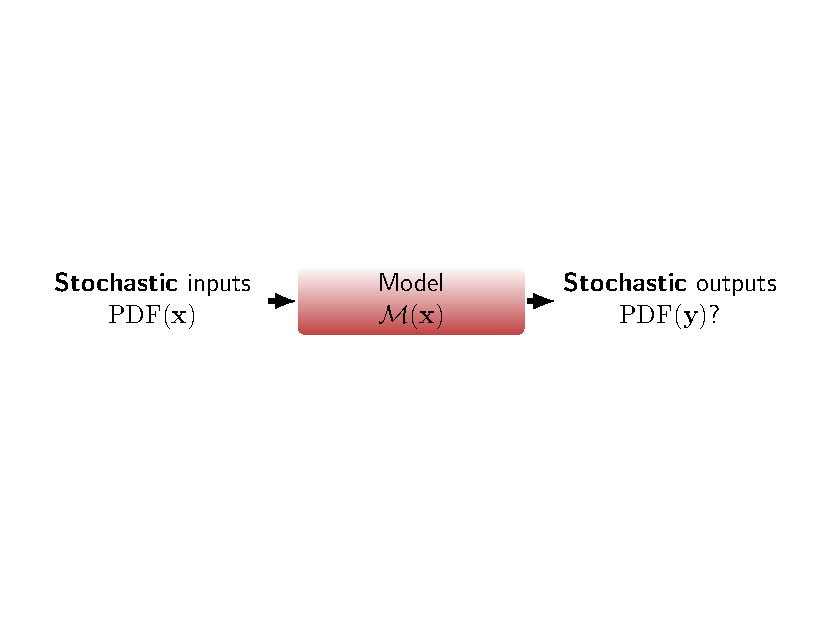
\includegraphics[width=22pc]{Figures/0_problem_statement.pdf}
\caption{Uncertainty propagation problem diagram.}
\label{fig_UQ_problem}
\end{centering}
\end{figure}


\subsection{Solution overview}


Polynomial chaos expansion (PCE) is a methodology used to efficiently propagate input uncertainties through a non-linear model. This methodology consists in building a polynomial response surface to capture the global dependency of the output as a function of the uncertain inputs. In particular, polynomial chaos expansions uses a set of polynomials that have special properties with respect to the probability distribution of the input variables. This makes the PCE an efficient method to obtain the statistics of the output without requiring an additional Monte-Carlo simulation using the surrogate. PCE is a technique widely used in the uncertainty quantification field because of its simplicity and fast convergence in comparison to a full Monte-Carlo simulation based on the original model \cite{soize2004physical, le2004uncertainty, choi2004polynomial, berveiller2006stochastic, xiu2005high, blatman2011adaptive}.

Several open source implementations of PCE methods are available such as: Chaospy \cite{feinberg2015chaospy}, Dakota \cite{eldred2007dakota}, UQLab \cite{marelli2014uqlab} and OpenTurns \cite{andrianov2007open}. In the present work we use Chaospy because of its implementation of the Rosenblatt transformation. Additionally, the present work uses the solvers of the least absolute shrinkage and selection operator (LASSO) problem \cite{tibshirani1996regression} and the cross-validation capabilities available in Scikit-learn \cite{pedregosa2011scikit}. These capabilities are used inside of Chaospy for general users and were used externally in the present study to gain control over the different stages of cross-validation.

Two different variable transformations are applied to the variables in the present problem. The Rosenblatt transformation \cite{rosenblatt1952} is used to de-correlate the joint input distribution, $\pdf(\vx)$. The input variables are transform into independent uniform distributed variables in the unitary space, $\pdf(\vw)$. This means that only the Legendre polynomials are used in the uncorrelated uniform space. A logistic transformation \cite{simard1998transformation} is applied to every output variable to avoid overshooting of the polynomial surrogates. This last transformation enables the use of polynomial surrogates in problems with discontinuities and under strict constrains. The power production of a turbine is an example of an output variable with a discontinuity at the rated power which makes it difficult to surrogate without a transformation of variables.

% An example of constrained surrogates are the surrogates for the local standard deviation $\hat{y}_{\std}(\vx)$, which are constrained to be positive over all the input space.

\begin{figure}[h!]
\begin{centering}
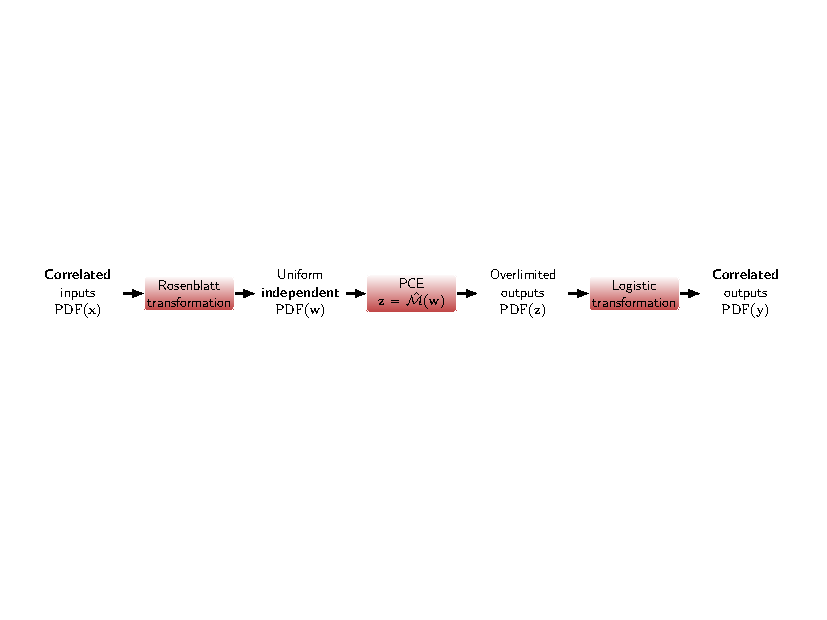
\includegraphics[width=\columnwidth]{Figures/2_transfromation_steps.pdf}
\caption{Model diagram.}
\label{fig_HR_loc}
\end{centering}
\end{figure}



%\section{Cases:}
%\subsection{DTU 10 MW RWT}
\section{DTU 10 MW RWT}

The model consist of the DTU 10 MW reference wind turbine HAWC2 model \cite{larsen20072, bak2012light} with Mann turbulent inflow generation \cite{Mann1998}. The joint input distribution is defined for a Class I-B site using four variables ($\vx=[\ws,\stdws,\shear,\yaw]^T$): 10 minutes mean wind speed ($\ws$ in m.s$^{-1}$), 10 minutes standard deviation of the wind speed in the streamwise velocity ($\stdws$ in m.s$^{-1}$), 10 minute mean shear exponent ($\shear$) and 10 minutes mean yaw miss-alignment ($\yaw$ in $^{\circ}$). The joint input distribution $\pdf(\vx)$ is based on the joint distribution defined by Dimitrov et al \cite{dimitrov2015model}. The Rosenblatt transformation is used to transform the correlated variables to an uncorrelated unitary uniform space \cite{rosenblatt1952}.

\begin{figure}[h!]
\begin{centering}
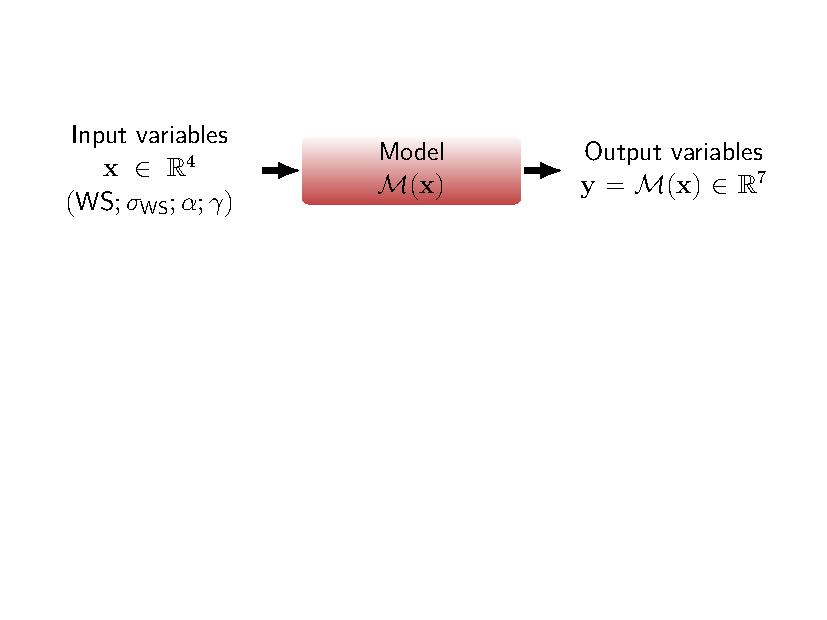
\includegraphics[width=22pc]{Figures/1_HAWC2_UQ_problem.pdf}
\caption{Model diagram.}
\label{fig_HR_loc}
\end{centering}
\end{figure}

\eq{\begin{split}
\ws & \sim \text{Weibull}(k = 2, A = 10/\Gamma(1+1/k), low = 4, high = 25) \\
\stdws & \sim \text{Lognormal}(\mu_{\stdws} = \mu_{\stdws}(\ws), \sigma_{\stdws} = \sigma_{\stdws}(\ws)) \\
\shear & \sim \text{Normal}(\mu_{\shear} = 0.088[Ln(\ws) - 1], \sigma_{\shear} = 1/\ws) \\
\yaw & \sim \text{Normal}(\mu_{\yaw}=0, \sigma_{\yaw}= 5)
\end{split}
}{eq_pdf_input}

The dependency between $\ws$ and $\stdws$ is defined in terms of the mean and variance of $\stdws$ in the Normal Turbulence Model described in the IEC 61400-1 \cite{international2005iec}. This dependency is not given in terms of the parameters of the Lognormal distribution ($\mu_{\stdws}$, $\sigma_{\stdws}$).

\eq{
\begin{split}
\variance(\stdws|\ws) &= Ln( 1 + 1.4^2/[0.75 \ws + 3.8]^2) \\
\expect(\stdws|\ws) & = Ln( \text{TI}_{\text{ref}}[0.75 \ws + 3.8] ) - \variance(\stdws|\ws)/2 \\
\end{split}
}{}

Multiple random turbulent inflow fields that share the same input variables ($\vx$) can be obtained using different seeds in the random turbulent flow generation process \cite{Mann1998}. This article considers the uncertainty due to limited number of turbulent inflow seeds required to build accurate surrogates.

Seven different model outputs are considered ($\vy$): 10 minute mean power production ($P$ in $\times 10$ MW), 10 minute mean thrust coefficient (CT), damage equivalent fatigue load for the flapwise blade root bending moment for a M{\"o}hler material coefficient of 12 (BRFBM\_EFL\_M12 in MN.m), damage equivalent fatigue load for the fore-aft tower bottom bending moment (TBFBM\_EFL\_M4 in MN.m), damage equivalent fatigue load for the sidewise tower bottom bending moment (TBSBM\_EFL\_M4 in MN.m), damage equivalent fatigue load for the tilt tower top bending moment (TTTBM\_EFL\_M4 in MN.m), damage equivalent fatigue load for the yaw tower top bending moment for a M{\"o}hler material coefficient of 4 (TTYBM\_EFL\_M4 in MN.m).

The equivalent fatigue loads are computed using a rainflow counting algorithm given in the equation \ref{eq_EFL} by Miner et al \cite{miner1945cumulative}. The number of load cycles $n_i$ with a load range $S_i$ are weighted using different material's M{\"o}hler coefficient $m$. The equivalent fatigue loads correspond to a 1 Hz vibration during the 10 minutes, therefore the reference load number $N_{\text{ref}}$ is 600.

\eq{S_{\text{eq}} = \left( \frac{\sum n_i S_i^m}{N_{\text{ref}}} \right)^\frac{1}{m}}{eq_EFL}

In the present study, two outputs are considered for each variable: the mean of the output with respect the multiple turbulent inflow repetitions (turbulent seeds) $y_{\expect}(\vx)=\expect(y|\vx)=\sum y_i(\vx)/N_{\text{seeds}}$ and the standard deviation of the output with respect the turbulent inflow $y_{\std}(\vx)=\std(y|\vx)=[\sum [y_i(\vx) - y_{\expect}]^2/[N_{\text{seeds}}-1]]^{1/2}$. Note that this decomposition is the local distribution for a given input point ($\vx$) resulting from the stochasticity of the turbulent inflow field: an aeroelastic model does not return the same value of a given output for the same input conditions ($\vx$) if the turbulent inflow realization is different. The decomposition can be understood as an uncertainty model due to the turbulent inflow: $y_{PCE}(\vx) \sim \text{Normal} (\hat{y}_{\expect}(\vx),\hat{y}_{\std}(\vx))$.

\section{Methodology}

\subsection{1D PCE theory}

Consider a model with a single uncertain input variable $x$ and a single output $y$. One can define a family of polynomials $\poly_l (x)$ to be used to approximate the output function. Where the order of each polynomial is given by $l$. In most cases the family of polynomials used for response surface approximation is the natural family ($1$, $x$, $x^2$, $\dots$). In general if the family of polynomials does not consider any information about the distribution of the input this approximation is a referred to as a polynomial response surface:

\eq{y(x) \approx \sum\limits_{l = 0}^{M} c_l \, \poly_l (x)}{}

PCE consist in defining a polynomial family that is orthogonal with respect the input distribution. It is then required to define an inner product between two arbitrary functions, $f(x)$ and $g(x)$ with respect the probability density function of the input $\pdf(x)$ as:

\eq{\langle  f, g \rangle  =\int f(x)\,g(x)\, \pdf(x)\,dx}{}

The polynomial basis ($\phi_{i}$ for polynomial orders $i=0,1,\dots$) is then constructed such that $\phi_{0}=1$ and all the polynomials are orthogonal:

\eq{\langle  \phi_{l},\phi_{k} \rangle = \delta_{lk} = \begin{cases}
                        1 \text{ if $l=k$} \\
                        0 \text{ if $l \neq k$}
                    \end{cases}}{}

An important consequence of the orthogonality property is that all the polynomials in the orthogonal basis are orthogonal to the unitary function:

\eq{\langle 1, \phi_{l} \rangle = 0 \quad \forall l>0 \quad \iff \quad \int \phi_{l}(x)\, \pdf(x)\,dx = 0 \quad \forall l>0}{}

Note that since the polynomials are of increasing order they can still be used to build a polynomial approximation of the output. i.e. a polynomial response surface. Where, $c_l$ are the coefficients (coordinates) correspondent to each of the elements of the polynomial basis.

\eq{y(x) \approx \sum\limits_{l = 0}^{M} c_l \, \phi_{l} (x)}{}

The orthogonality property makes the PCE particularly useful approach to propagate uncertainty over polynomial response surface because the statistical moments of the output can be derived directly from the coefficients.

\eq{\expect(y) = \int y(x)\, \pdf(x)\,dx  = \langle 1, y \rangle \approx \langle 1, \sum\limits_{l = 0}^{M} c_l \, \phi_{l} \rangle = \sum\limits_{l = 0}^{M} c_l \langle 1, \phi_{l} \rangle = y_{0}}{}

\eq{\expect(y^2) = \int y^2(x) \pdf(x)\,dx  = \langle y, y \rangle \approx \sum\limits_{l = 0}^{M} \sum\limits_{m = 0}^{M} c_l \, y_{m} \langle \phi_{l}, \phi_{m} \rangle = \sum\limits_{l = 0}^{M} y^2_{l}}{}

\eq{\variance(y) = \expect(y^2) - \expect(y)^2 =  \sum\limits_{l = 1}^{M} y^2_{l}}{}

The orthogonal polynomial families with respect the most important distributions have been determined and used in many research ares such as physics and mathematics, see table \ref{tab_poly}.

\begin{table}[h!]
\begin{center}
\resizebox{0.4\linewidth}{!}{
\begin{tabular}{ l c }
  Distribution & Polynomial Family \\
  \hline
  Uniform & Legendre \\
  Normal & Hermite \\
  Exponential & Laguerre
\end{tabular}}
\end{center}
\caption{Classical orthogonal polynomial families.}
\label{tab_poly}
\end{table}

There are two different approaches to determine the PCE coefficients: (1) \emph{Semi-Spectral projection} consists in using quadrature rules to approximate the inner product definition of the coefficient. Many quadrature rules exist to approximate the integrals; each quadrature gives $N_n$ nodes for model evaluation ($x_i$) and their corresponding weights ($\omega_i$). The coefficients are then obtained by projection:

\eq{c_l = \langle  y,  \phi_{l} \rangle  =\int y(x)\, \phi_{l}(x)\, \pdf(x)\,dx \approx \sum_{i=0}^{N_n} \omega_i \, y(x_i) \, \phi_{l}(x_i)}{}

Gaussian quadratures are widely used because they are very accurate for smooth function integration with respect a weight function (in this case the $\pdf(x)$). In general semi-spectral projection is very accurate method for low number of dimensions, but the number of model evaluations required grows exponentially with the number of dimensions. Additionally, quadrature rules can be unstable for heavy tailed PDFs.

(2) \emph{Point collocation} consists in fitting the polynomial basis to a small sample of model evaluations. Traditionally, this fit can be done using least squares algorithm, but some other optimization algorithms can also be used such as least angle regression (LAR) \cite{blatman2011adaptive}. In general point collocation is very robust and the advanced optimization algorithms are designed to handle large number of dimensions, to avoid over-fitting and to achieve sparsity in the final surrogate (to reduce the number of active terms). The present study focuses only in point collocation techniques since the number of model required to obtain a sparse PCE is smaller.

\subsection{Multiple dimension PCE}

To build the PCE of a model with correlated multiple input dimensions ($\vx$), it is required to initially transform the correlated input space into an uncorrelated space ($\vw$). This transformation enables the use of variance reduction Monte-Carlo sampling techniques to define the training points of a surrogate \cite{feinberg2015chaospy}. Additionally, the multidimensional polynomial basis is just the product of the unidimensional polynomials for each of the uncorrelated variables. In this article the Rosenblatt transformation \cite{rosenblatt1952} is used due to the fact that the input distribution is defined in a sequence of conditional relationships. The Rosenblatt transformation consists on using the cumulative density function CDF of each individual variable, in sequence, to transform the variable into an uncorrelated uniform distribution: $R(\vw)=\vx$. This means that the PCE for the applications shown in this article only use standard Legendre polynomials, $y(\vx)\approx \hat{y}(\vw)$. An example of the Rosenblatt transformation is shown in figure \ref{fig_rosen}.

\begin{figure}[h!]
\begin{centering}
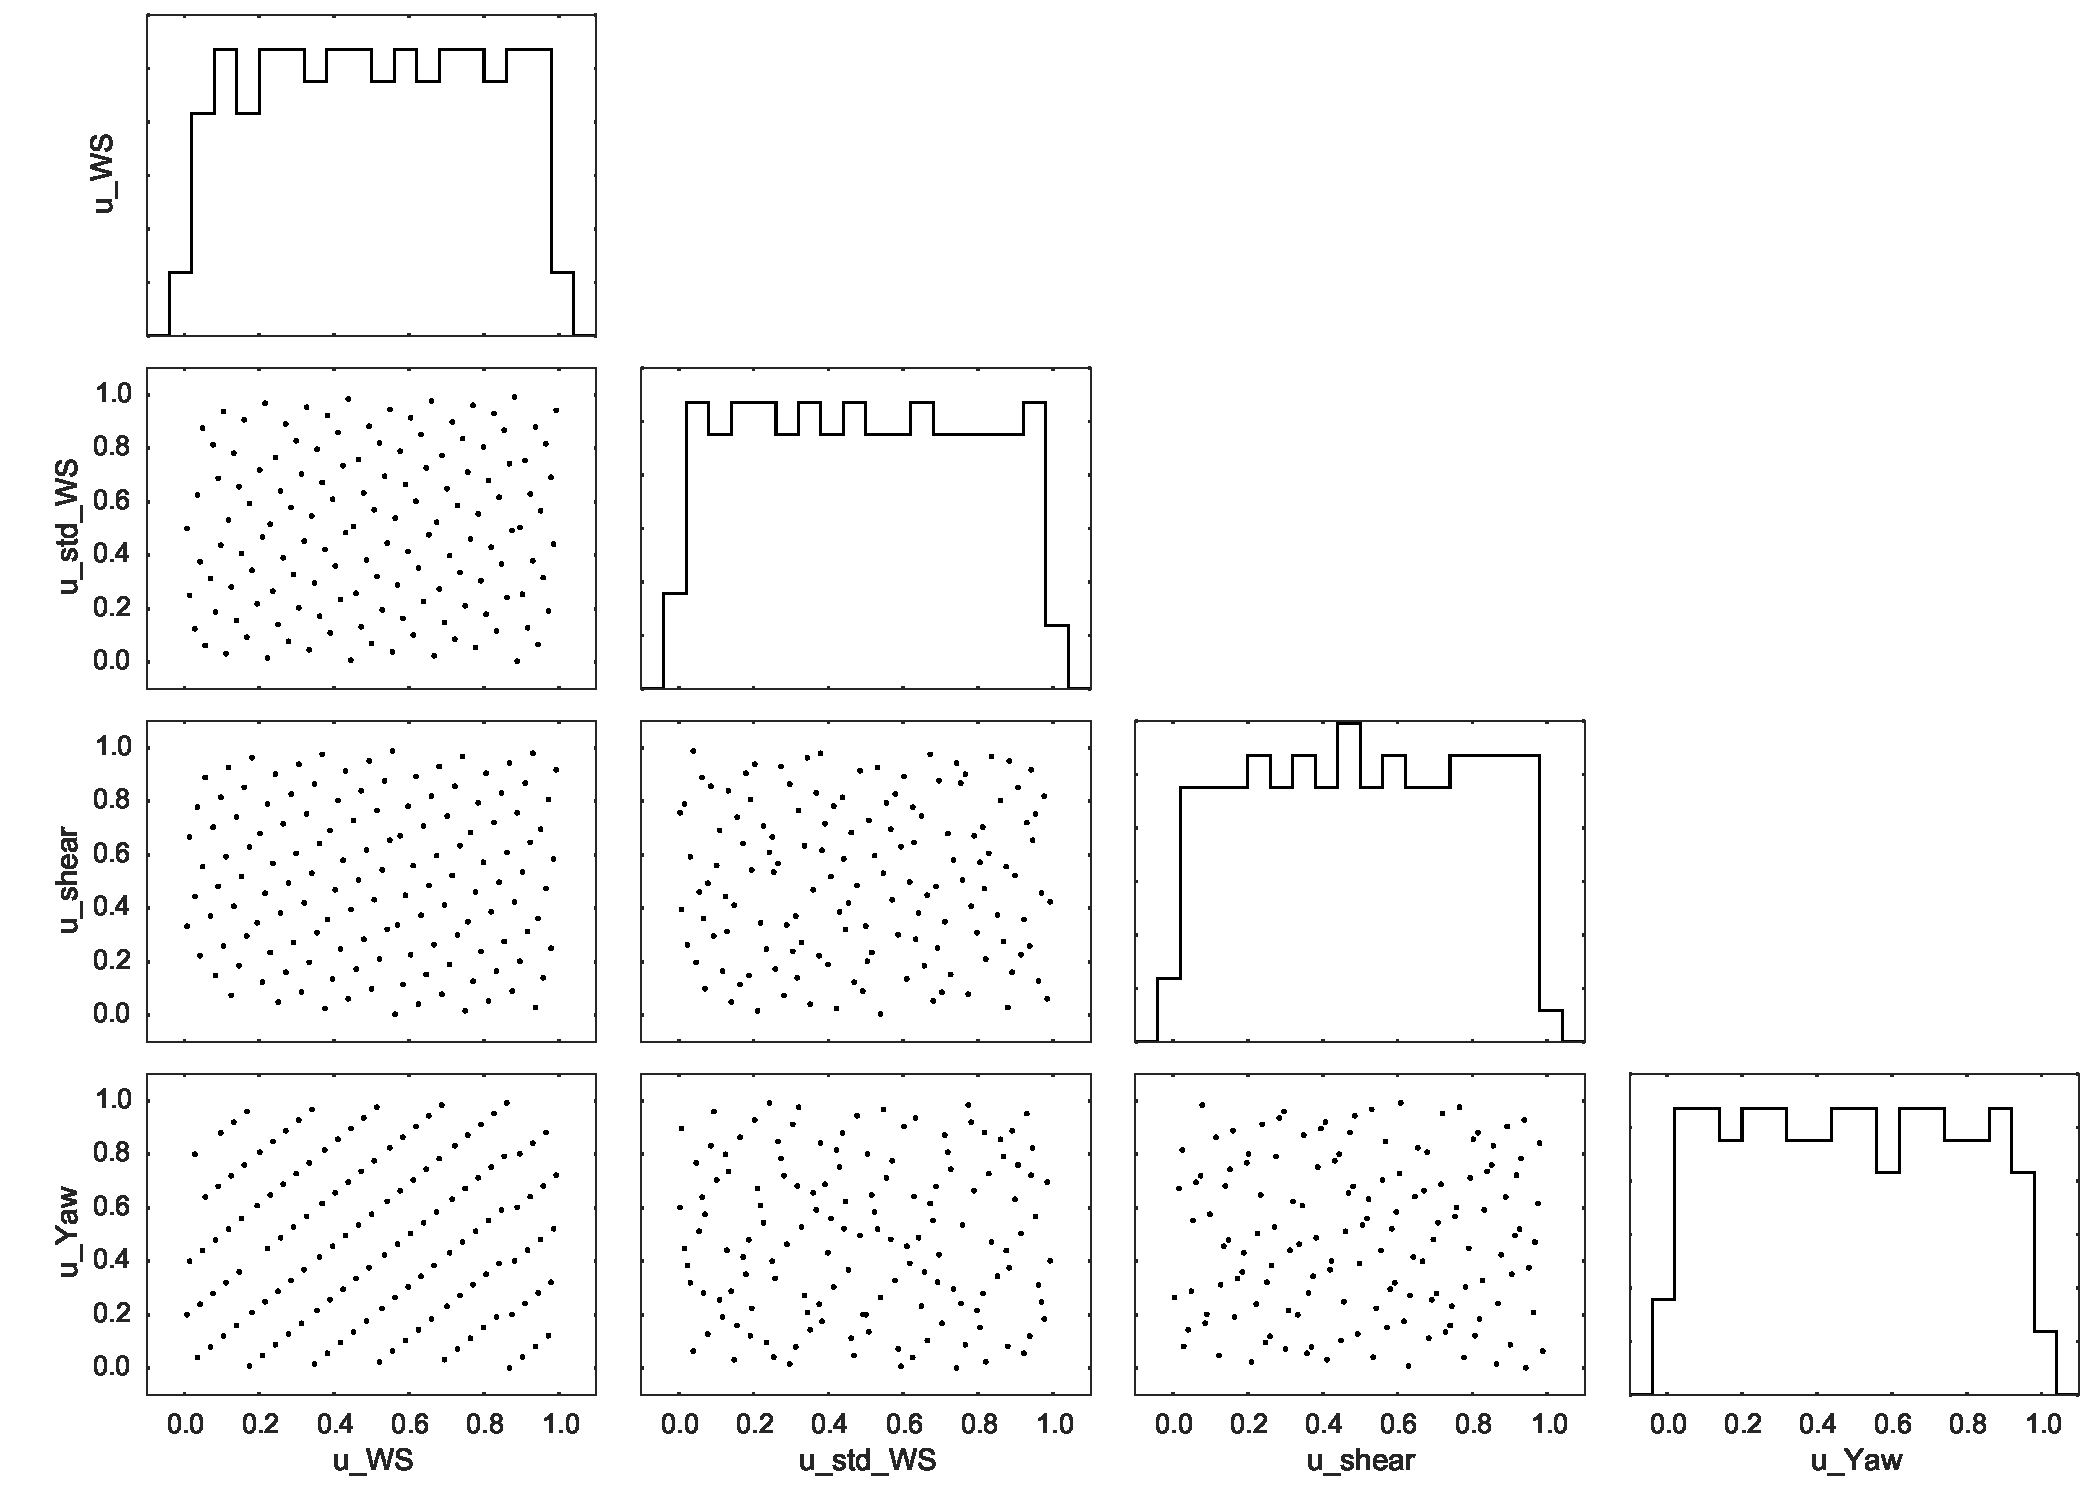
\includegraphics[width=0.48\columnwidth]{Figures/PCE_train_x_Unif.pdf}
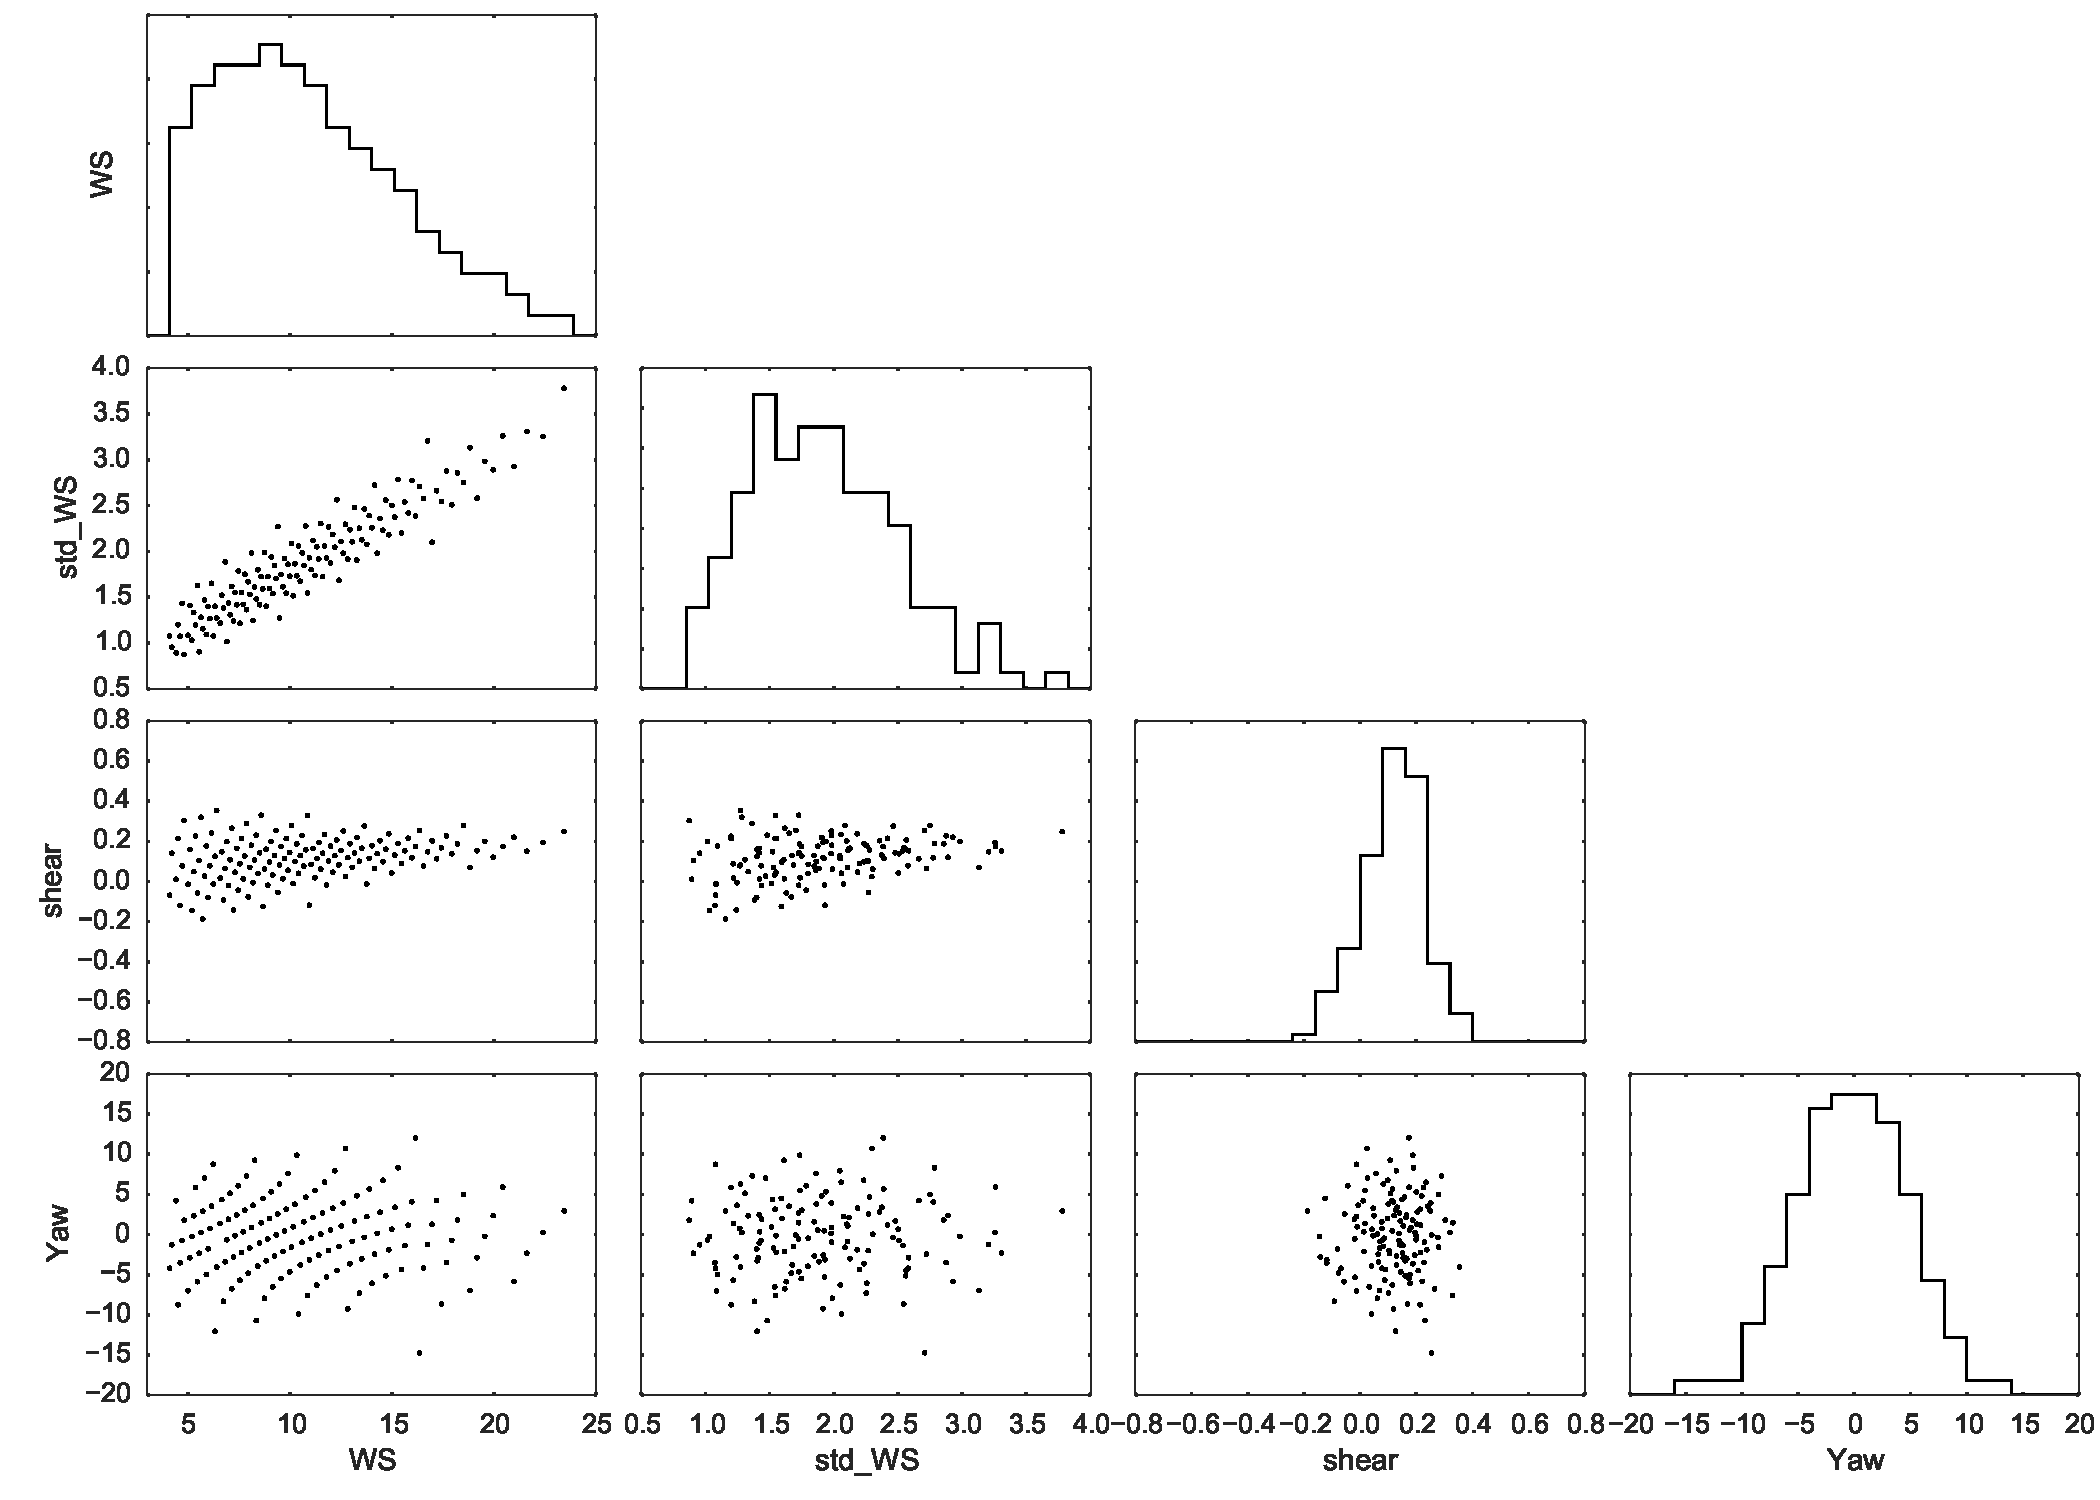
\includegraphics[width=0.48\columnwidth]{Figures/PCE_train_x.pdf}
\caption{(Left) Sample in the uncorrelated uniform space $\pdf(\vw)$. (Right) Same sample transformed into the correlated input space $\pdf(\vx)$.}
\label{fig_rosen}
\end{centering}
\end{figure}

The $D$-dimensional polynomial is constructed as the product between 1D polynomials. A $D$-dimensional polynomial of the independent uniform variables $\vw=[w_0,\dots,w_D]$ is written using the set of multiple indexes: $\multind \subset \mathbb{N}^D$, where an element $j\in \multind$ contains the order of the polynomial in each dimension $j = [l_0, \dots, l_D]$:

\eq{y(\vx) = y(R(\vw)) \approx \sum\limits_{j \in \multind} c_{j} \, \mpoly_{j} (\vw)}{}

and an element in the multidimensional polynomial basis is given as:

\eq{\mpoly_{j} (\vw) =  \phi_{l_0}(w_0) \times \dots \times \phi_{l_D}(w_D)}{}

Global sensitivity analysis characterized by the Sobol's indices based on variance decomposition can also be calculated using only the coefficients of the PCE \cite{sudret2008global}. The total effect sensitivity analysis represents the amount of variance in the output that is described by all the terms that include effects on that variable.

\eq{S_{\text{total}\,y,x_k} = \frac{\variance(y|j \in \multind \,\&\, l_k>0)}{\variance(y)} =  \frac{\sum\limits_{j \in \multind \,\&\, l_k>0} c_{j}^2}{\sum\limits_{j \in \multind \,\&\, j\neq[0,0,0,0]} c_{j}^2} }{}

\subsection{Training point selection}

If the total polynomial order is truncated to be smaller than an order M. Then the number of terms, and therefore of unknown coefficients, $N_c$ is:

\eq{N_c = \left( \begin{array}{c} M + D \\ M \end{array} \right)}{}

In order to avoid over-fitting and to have extra model evaluations to test the accuracy of the surrogate the total number of model evaluations is suggested to be between 2 or 3 times the number of unknowns \cite{blatman2011adaptive}. In this article the number of evaluations are set to be $N=2\,N_c$, and the maximum order of the polynomial is expected to be 4. Note that this maximum order is only used to estimate the number of model evaluations; the final regression technique used allows to explore higher order terms \cite{tibshirani1996regression, blatman2011adaptive}. This leads to an estimated number of model evaluations of 140 for the DTU 10 MW RWT case and of 252 for the NREL 5 MW RWT case. A Hammersley sequence \cite{hammersley1960monte} is used to generate the training sample as suggested by Feinberg and Hosder  \cite{feinberg2015chaospy, hosder2007efficient}.

\begin{figure}[h!]
\begin{centering}
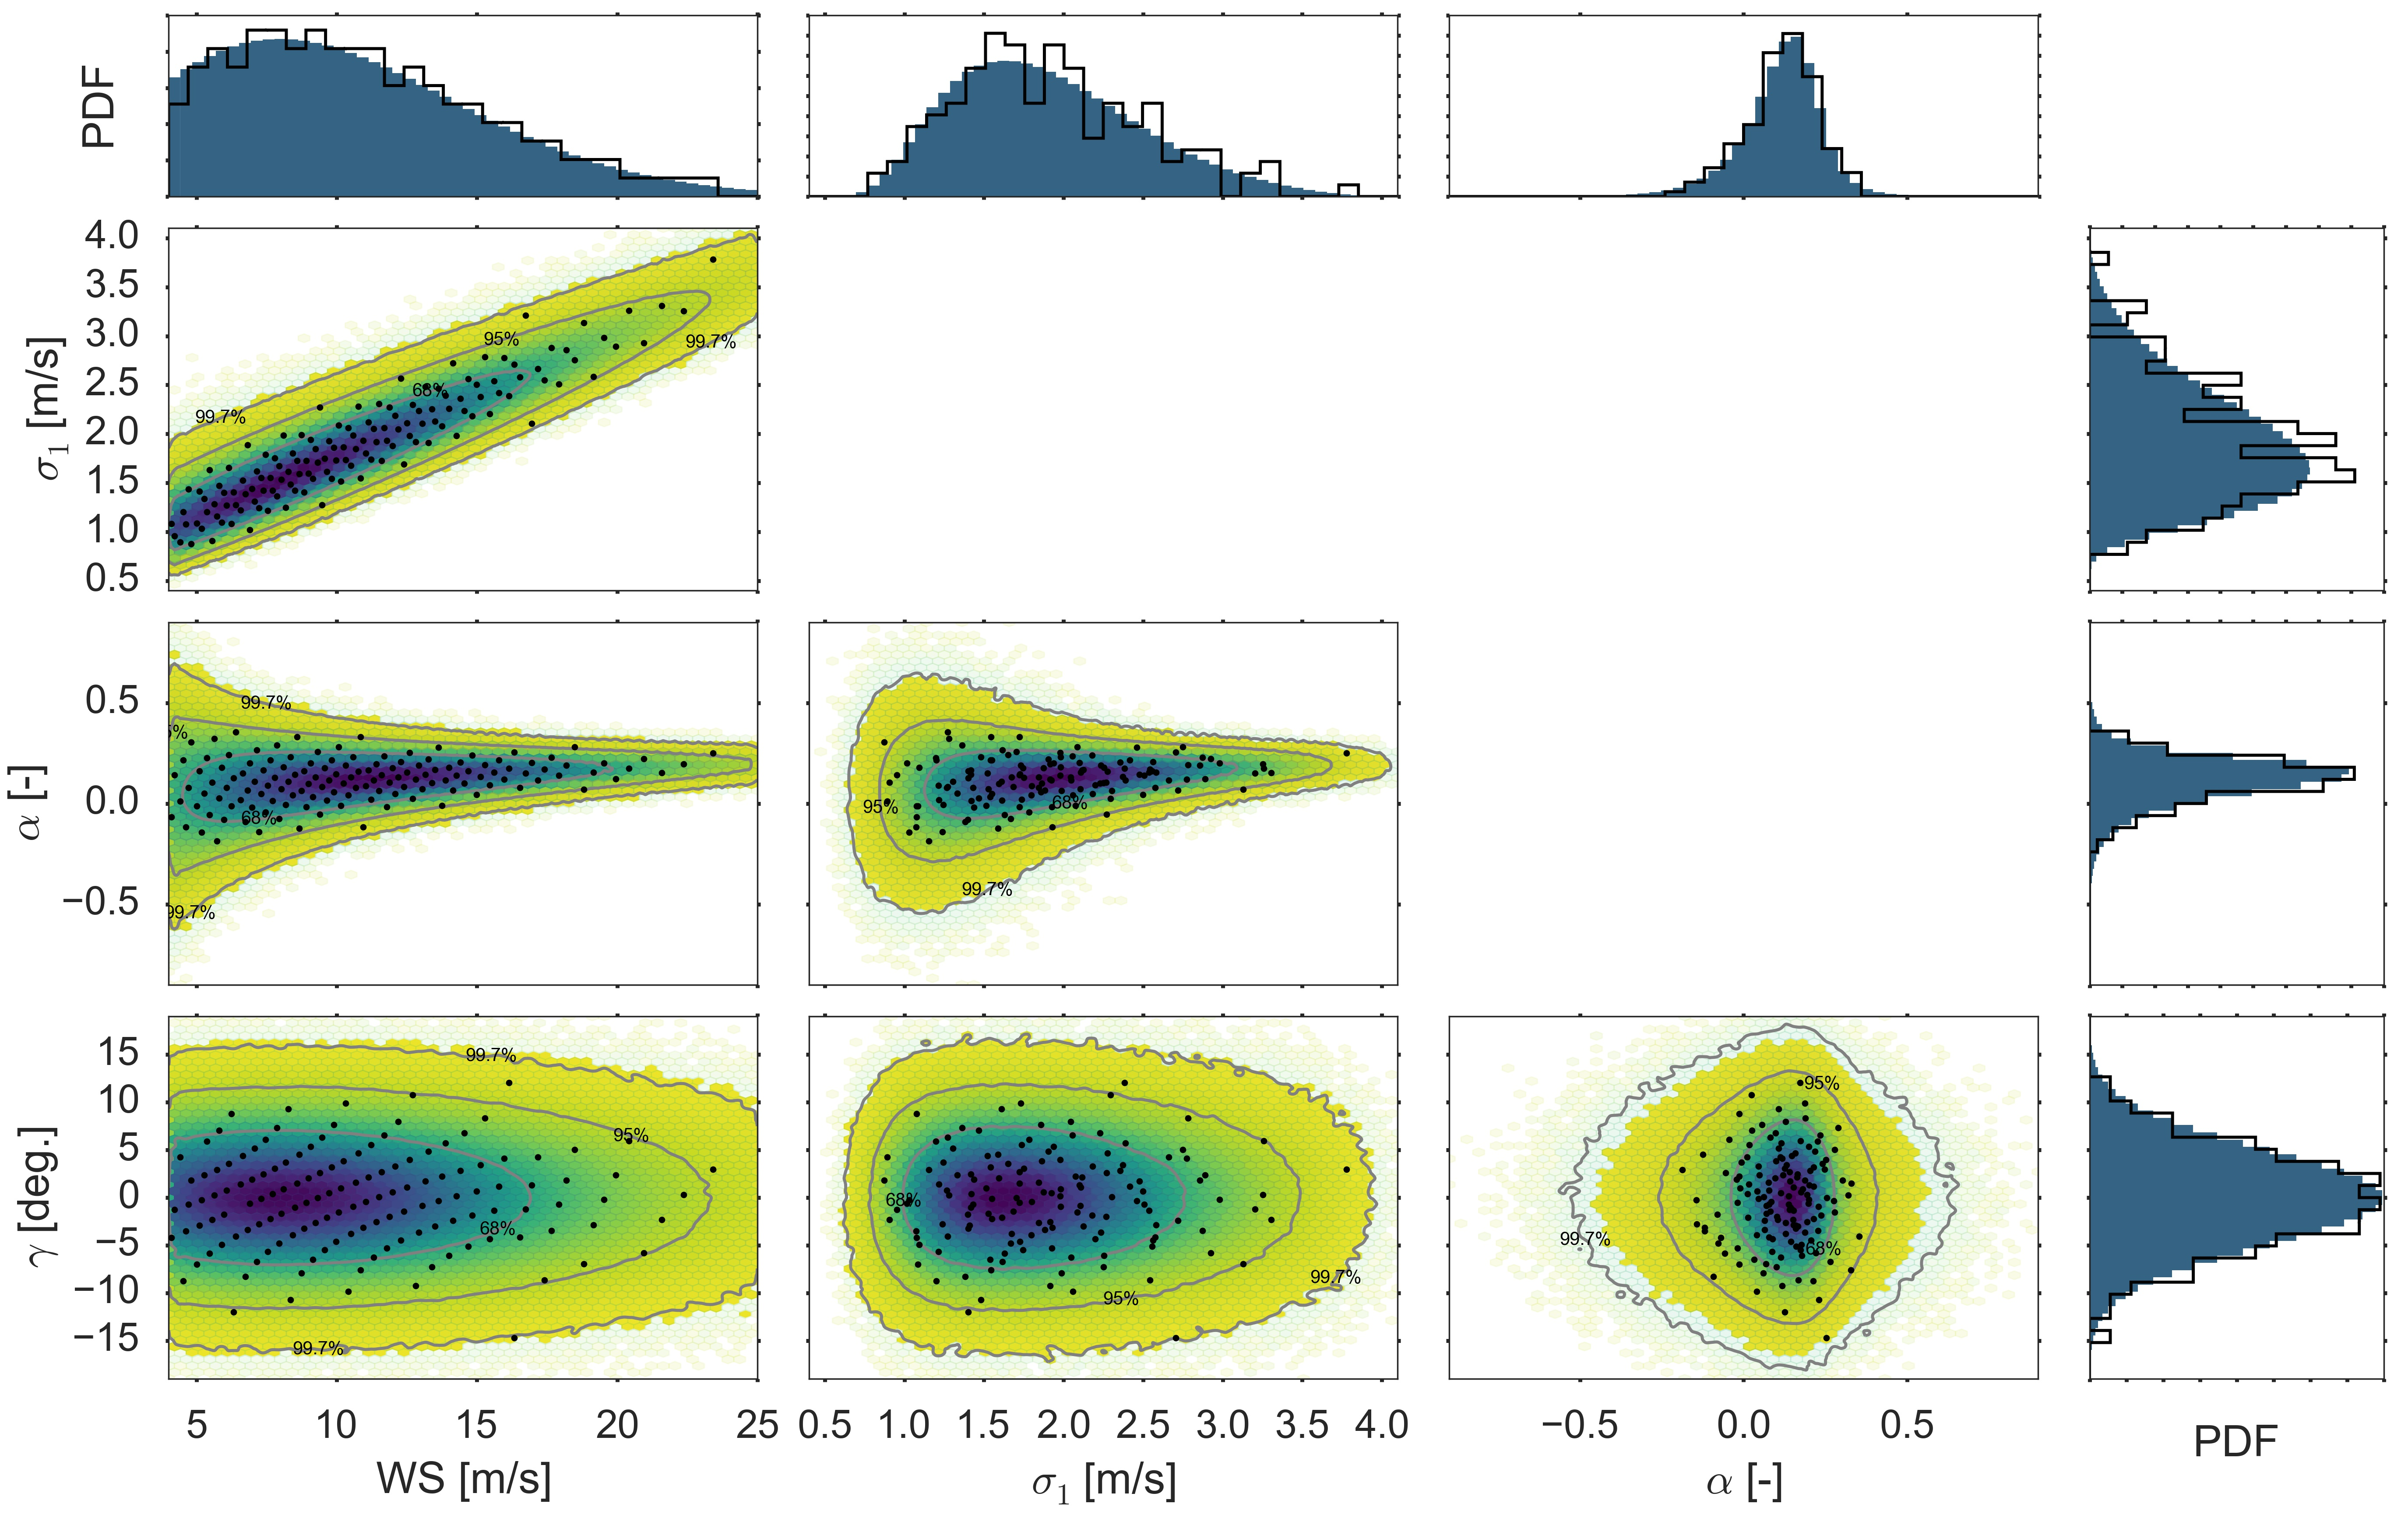
\includegraphics[width=0.8\columnwidth]{Figures/PCE_train_x_full.pdf}
\caption{(Black points) Training dataset in the inputs: 140 Hammersley sequence sample of input joint distribution. (Histogram colored hex-bins) 80000 Hammersley sequence sample Monte-Carlo sample.}
\label{fig_PCE_train_x_full}
\end{centering}
\end{figure}

\subsection{Logistic transformation}

A logistic transformation is applied to every output of the model in order avoid over-shotting, and hence to impose strict restrictions to the polynomial surrogates. This transformation uses the logit function $L(p)=Ln(p/(1-p))$ and its inverse, the logistic function $L^{-1}(p) = 1/(1+e^{-p})$, to transform the actual outputs ($\vy$) into a smooth and possibly over-shooting variable space ($\vz$) \cite{simard1998transformation}. The constants of the transformation ($a_k$ and $k_k$) are calibrated for each of the variables $y_k$ in order to impose constrains that agree with the expected behavior of the output and to avoid numerical instabilities. See equations \ref{eq_logistic} and \ref{eq_logit}.

\eq{z_k = L(k_k\,y_k+a_k)}{eq_logistic}

\eq{y_k = \frac{L^{-1}(z_k) - a_k}{k_k} }{eq_logit}

\begin{table}[!h]
\begin{centering}
\resizebox{0.5\linewidth}{!}{
\begin{tabular}{c|cc}
Output &       $k_k$ &       $a_k$ \\
\hline
P\_E             & $9.5\times10^{-1}$ &  $0.0$ \\
CT\_E            & $1.0$ & $-5.0\times10^{-2}$ \\
BRFBM\_EFL\_M12\_E & $2.2\times10^{-2}$ &  $0.0$ \\
TBFBM\_EFL\_M4\_E  & $1.0\times10^{-2}$ &  $0.0$ \\
TBSBM\_EFL\_M4\_E  & $1.4\times10^{-2}$ &  $0.0$ \\
TTTBM\_EFL\_M4\_E  & $3.3\times10^{-2}$ &  $0.0$ \\
TTYBM\_EFL\_M4\_E  & $3.3\times10^{-2}$ &  $0.0$ \\
P\_S             & $5.0$ &  $1.0\times10^{-4}$ \\
CT\_S            & $5.0$ &  $1.0\times10^{-4}$ \\
BRFBM\_EFL\_M12\_S & $1.7\times10^{-1}$ &  $1.0\times10^{-4}$ \\
TBFBM\_EFL\_M4\_S  & $2.5\times10^{-2}$ &  $1.0\times10^{-4}$ \\
TBSBM\_EFL\_M4\_S  & $2.5\times10^{-2}$ &  $1.0\times10^{-4}$ \\
TTTBM\_EFL\_M4\_S  & $1.7\times10^{-1}$ &  $1.0\times10^{-4}$ \\
TTYBM\_EFL\_M4\_S  & $1.7\times10^{-1}$ &  $1.0\times10^{-4}$
\end{tabular}}
\label{tab_logistic}
\caption{Logistic transformation constants for each output.}
\end{centering}
\end{table}

\subsection{LASSO problem}

The least absolute shrinkage and selection operator problem \cite{tibshirani1996regression} is a modified least squares optimization problem that adds a term that penalizes the sum of the absolute values of all coefficients ($\ell_1$ norm regularization term).

\eq{\min_\vc ||\vc \boldsymbol{\Phi} - \text{\textbf{y}}_k||^2_2 + \alpha_k ||\vc||_1 = \min_\vc \sum_{i=0}^{N-1} \left[ \sum_{l=0}^{N_c-1} c_l \mpoly_l(\vw_i) - y_k(\vx_i) \right]^2 + \alpha_k \sum_{l=0}^{N_c-1} |c_l|}{}

LASSO is used to achieve sparsity in the final polynomial surrogate, which translates in minimizing the number of active members of the polynomial base. In general, LASSO prefers solutions with the least number of active terms. There are two algorithms available in Scikit-learn to solve the LASSO problem \cite{pedregosa2011scikit}: coordinate descent and least angle regression. The regularization coefficient $\alpha_k$ controls the amount of active terms in the final solution. Smaller values allow to have more active terms while larger values will prefer final surrogates with very few active terms.

\subsection{k-Fold cross-validation for optimization of LASSO regularization}


The present study uses Scikit-learn cross-validation capabilities \cite{pedregosa2011scikit}. Cross-validation is used to optimize the regularization coefficient $\alpha_k$ in order to avoid over fitting of the data. The coordinate descend algorithm available in Scikit-learn is used to solve the LASSO problem because it receives a range of regularization coefficients instead of exploring the full space of $\alpha_k$'s as the least angle regression (LAR) algorithm does. The k-fold cross-validation consists in splitting the dataset into k groups of data. k-1 of the groups are used for training and the remaining one is used for cross-validation. The surrogate fitted using k-1 groups is used to predict the output observed in each of the element in the remaining group. The error in the prediction of the surrogate can then be computed. This process is repeated for each individual fold and for multiple regularization parameters. The regularization parameter that gives the best mean cross-validation sum of errors is then selected to train the whole dataset. A 20-fold cross-validation is used to select the proper level of sparsity in each of the output. Examples of this cross-validation process are shown in figure \ref{fig_20fold}.

\begin{figure}[h!]
\begin{centering}
\includegraphics[width=0.3\columnwidth]{Figures/20Fold_CrossValidation_P_E_PCE.pdf} \includegraphics[width=0.3\columnwidth]{Figures/20Fold_CrossValidation_CT_E_PCE.pdf} \includegraphics[width=0.3\columnwidth]{Figures/20Fold_CrossValidation_BRFBM_EFL_M12_E_PCE.pdf}
\caption{Examples of the 20-Fold cross validation for the optimization of regularization coefficient. (Blue lines) Cross-validation mean square error for a different fold used as validation. (Black line) Mean of the 20 folds cross-validation mean square error. (Red line) Selected regularization parameter.}
\label{fig_20fold}
\end{centering}
\end{figure}


\subsection{Example of PCE surrogates for $\vy_{\expect}$ and $\vy_{\std}$}

In the present study two polynomial chaos expansion are built independently for each output variable: One for the local mean of the output $\hat{y}_{\expect}(\vx)\approx y_{\expect}(\vx)=\expect(y|\vx)$ and one for the local uncertainty characterized as a standard deviation of the output $\hat{y}_{\std}(\vx) \approx y_{\std}(\vx)=\std(y|\vx)$. Note that this decomposition is the local distribution for a given input point ($\vx$) resulting from the stochasticity of the turbulent inflow field. In order to make a prediction of the output in a new input point, then, the mean and the standard deviation surrogates are used to predict the normal distribution of the output due to the turbulent inflow at each input variable location: $y(\vx) \sim \text{Normal} (\hat{y}_{\expect}(\vx),\hat{y}_{\std}(\vx))$. This enables not only to capture the global behavior of the turbine under different inflow conditions but also to estimate the variability due to different turbulent inflow realizations. Some examples of such surrogates are shown in figure \ref{fig_y_hat_E_V}. Note that in this figure the variable $P_{\std}$ represents the standard deviation of 100 different 10-min averaged powers in which each one has a different turbulent inflow realization. It should not be confused with the standard deviation of the instantaneous power during the 10 minutes of simulation. The benefits of using the logistic transformation can be seen in figure \ref{fig_y_hat_E_V}, note that the PCE do not present Gibbs oscillations due to the inability to maintain a constant value for a large region of the inputs, as it can be seen for P\_E, for P\_S and CT\_S.

\begin{figure}[h!]
\begin{centering}
\includegraphics[width=\columnwidth]{Figures/P_E_MC_PCE.pdf} \\
\includegraphics[width=\columnwidth]{Figures/P_S_MC_PCE.pdf} \\
\includegraphics[width=\columnwidth]{Figures/CT_E_MC_PCE.pdf} \\
\includegraphics[width=\columnwidth]{Figures/CT_S_MC_PCE.pdf}
\caption{(Black points) Training dataset in the outputs: 140 Hammersley sequence sample of input joint distribution. (Histogram colored hex-bins) 20000 Monte-Carlo simulation on the PCE surrogates.}
\label{fig_y_hat_E_V}
\end{centering}
\end{figure}

\subsection{Sensitivity analysis}

The sensitivity analysis (SA) for the two components of the outputs are computed automatically from the coefficients of the PCE surrogates using the implementation available in Chaospy \cite{feinberg2015chaospy} of the expressions presented in Sudret et al \cite{sudret2008global}. The total effect Sobol indexes represents the amount of variation in the output that could be reduced if the input variable were to be fixed in  a single value. It represents the non-linear influence of the input variable in the total variance of the output. Most of the outputs have a large total Sobol index for the wind speed. $\ws$ is clearly the main variable to explain the power and loads in a wind turbine; in particular the SA shows that the local expected power and thrust coefficient can be explained only with $\ws$. This corroborates the use of power and thrust coefficient curves by the wind industry. The $\stdws$ becomes important for the local expected value of the loads and for the uncertainty components of the outputs (the local standard deviation of the outputs). The shear and yaw have reduced effects over most variables. The shear exponent becomes important only for the fatigue due to blade root bending moment (BRFBM\_EFL\_M12); while the yaw miss alignment becomes important for the local variation of the fatigue due to the tower bottom fore-aft moment (TBFBM\_EFL\_M4\_S) and the tower top tilt moment (TBFBM\_EFL\_M4\_S).

\begin{table}[!h]
\begin{centering}
\resizebox{0.7\linewidth}{!}{
\begin{tabular}{c|cccc}
Output &      $\ws$ &  $\stdws$ &   $\shear$ &     $\yaw$ \\
\hline
P\_E             & $1.0$ & $2.3\times10^{-4}$ & $3.1\times10^{-4}$ & $9.6\times10^{-5}$ \\
P\_S             & $9.9\times10^{-1}$ & $1.2\times10^{-2}$ & $4.8\times10^{-3}$ & $5.5\times10^{-3}$ \\
\hline
CT\_E            & $1.0$ & $1.4\times10^{-3}$ & $1.6\times10^{-3}$ & $7.7\times10^{-4}$ \\
CT\_S            & $9.9\times10^{-1}$ & $1.5\times10^{-2}$ & $3.0\times10^{-4}$ & $2.6\times10^{-4}$ \\
\hline
BRFBM\_EFL\_M12\_E & $9.4\times10^{-1}$ & $5.8\times10^{-2}$ & $1.4\times10^{-2}$ & $3.1\times10^{-3}$ \\
BRFBM\_EFL\_M12\_S & $7.8\times10^{-1}$ & $2.2\times10^{-1}$ & $1.9\times10^{-2}$ & $1.7\times10^{-3}$ \\
\hline
TBFBM\_EFL\_M4\_E  & $7.4\times10^{-1}$ & $3.0\times10^{-1}$ & $3.7\times10^{-4}$ & $1.2\times10^{-3}$ \\
TBFBM\_EFL\_M4\_S  & $9.3\times10^{-1}$ & $7.0\times10^{-2}$ & $1.5\times10^{-3}$ & $3.7\times10^{-3}$ \\
\hline
TBSBM\_EFL\_M4\_E  & $9.2\times10^{-1}$ & $9.7\times10^{-2}$ & $1.9\times10^{-3}$ & $1.8\times10^{-4}$ \\
TBSBM\_EFL\_M4\_S  & $9.3\times10^{-1}$ & $6.8\times10^{-2}$ & $5.8\times10^{-3}$ & $1.7\times10^{-3}$ \\
\hline
TTTBM\_EFL\_M4\_E  & $9.2\times10^{-1}$ & $8.1\times10^{-2}$ & $4.0\times10^{-4}$ & $6.9\times10^{-4}$ \\
TTTBM\_EFL\_M4\_S  & $7.6\times10^{-1}$ & $2.5\times10^{-1}$ & $6.1\times10^{-3}$ & $7.5\times10^{-3}$ \\
\hline
TTYBM\_EFL\_M4\_E  & $9.3\times10^{-1}$ & $7.4\times10^{-2}$ & $2.6\times10^{-4}$ & $7.6\times10^{-4}$ \\
TTYBM\_EFL\_M4\_S  & $8.2\times10^{-1}$ & $1.9\times10^{-1}$ & $2.9\times10^{-4}$ & $9.8\times10^{-4}$
\end{tabular}}
\label{tab_sens}
\caption{Total sensitivity indexes (Total influence Sobol indices).}
\end{centering}
\end{table}

\section{Results}

%\subsection{Case: DTU 10 MW RWT}

The figure \ref{fig_final_surrogates} shows the final surrogates of the DTU 10 MW RWT. These surrogates were obtained using the 140 input sample (Figure \ref{fig_PCE_train_x_full}) with 100 independent turbulent realization per input point. It can be observed that the amount of local output variation due to the turbulent inflow realization varies between outputs and depends on the region of the input space: each see-through black point represents an individual realization of the turbulence. The effect of the turbulent inflow realization is more important for the fatigue loads. It can be observed that the final surrogate can be used to generate a sample that will cover the full space. The surrogates are robust enough to predict the frequency of occurrence of extreme values such as the distribution resulting from the input point with largest $\stdws$ (this point also has the largest $WS$). This point seems to be outside the main trend in $\ws$ because it has a large $\stdws$ and $\shear$ given its $WS$. Note that the local distribution of this point is captured in the $\stdws$ trend. One of the main limitations of the present surrogates is that the local distribution of the output is assumed to be Normal. This is not true in reality and it is the result of having a wind turbine controller that has a different goal in each region.

\begin{figure}[h!]
\begin{centering}
\includegraphics[width=\columnwidth]{Figures/Full_surrogate/P_PCE_MC_surrogate.png} \\
\includegraphics[width=\columnwidth]{Figures/Full_surrogate/CT_PCE_MC_surrogate.png} \\
\includegraphics[width=\columnwidth]{Figures/Full_surrogate/BRFBM_EFL_M12_PCE_MC_surrogate.png} \\
\includegraphics[width=\columnwidth]{Figures/Full_surrogate/TBFBM_EFL_M4_PCE_MC_surrogate.png} \\
\includegraphics[width=\columnwidth]{Figures/Full_surrogate/TBSBM_EFL_M4_PCE_MC_surrogate.png} \\
\includegraphics[width=\columnwidth]{Figures/Full_surrogate/TTTBM_EFL_M4_PCE_MC_surrogate.png} \\
\includegraphics[width=\columnwidth]{Figures/Full_surrogate/TTYBM_EFL_M4_PCE_MC_surrogate.png}
\caption{(Black points) Training dataset in the outputs: 140 Hammersley sequence sample x 100 turbulent inflow realizations. (Histogram colored hex-bins) 80000 Monte-Carlo simulation on the PCE surrogates including turbulent flow realization estimation.}
\label{fig_final_surrogates}
\end{centering}
\end{figure}

\subsection{Convergence}

A leave-one-out (LOO) cross-validation is done to the combined surrogates (local expected and local uncertainty PCEs) to test the effect of the number of independent turbulent seeds required to obtain accurate predictions. This study also shows the convergence trends as a function of the number of independent turbulent inflow realizations. A LOO is equivalent as a k-fold validation in which the number of folds is equal to the number of data points. In this case the PCE methodology was applied to 139 input points with a different number of turbulent inflow realizations per inputs point. The prediction of the local distribution at the unused point is compared against full 100 realization observations. Three different validation metrics are used to compare the local distributions at the point left out for testing ($\vx_{LO}$): the relative error in the expected value ($CV_E$) (eq. \ref{eq_CV_EV}), the relative error in the standard deviation ($CV_E$) and the normalized area validation metric ($CV_A$), (eq. \ref{eq_CV_A}). The area validation metric gives the error between the empirical CDF based on the 100 turbulent realizations and the Normal distribution predicted by the PCE ($y_{PCE}(\vx) \sim \text{Normal} (\hat{y}_{\expect}(\vx),\hat{y}_{\std}(\vx))$). In this article, the area validation metric is normalized with respect the maximum scale of the output variable, in that way this error represent the fraction of the total scale that should be considered as extra uncertainty due to the statistical uncertainty due to limited number of simulations.

\eq{CV_E = \left| 1- \frac{\hat{y}_{\expect}(\vx_{LO})}{y_{\expect}(\vx_{LO})} \right| \quad \quad CV_S = \left| 1- \frac{\hat{y}^2_{\std}(\vx_{LO})}{y^2_{\std}(\vx_{LO})} \right|^{1/2}}{eq_CV_EV}

\eq{CV_A = \frac{\int_{-\infty}^{\infty} |CDF(y_{PCE}|\vx=\vx_{LO})-CDF_{emp}(y|\vx=\vx_{LO})|\, dy}{\max(y)}}{eq_CV_A}

The convergence of the validation metrics are shown for three different output in figure \ref{fig_convergence}. In this figure it can be seen that all the validation metrics converge as the number of turbulent inflow realizations per input are increased. Note that the LOO validation metric a distribution of the errors for multiple bootstraps (selecting the N turbulent seeds out of the possible 100 seeds available). The outliers are the extreme cases of selecting seeds with similar outputs in which the training local expected value and/or local standard deviation are not well predicted, in addition to the errors due to the PCE training/prediction and due to the assumption of local normality. The LOO cross validation for $P_S$ has a larger scale due to the fact that it is the only variable in which the observed standard deviation is exactly zero ($P_{\std}(\ws>15) = 0$), which makes the equation \ref{eq_CV_EV} divergent.

\begin{figure}[h!]
\begin{centering}
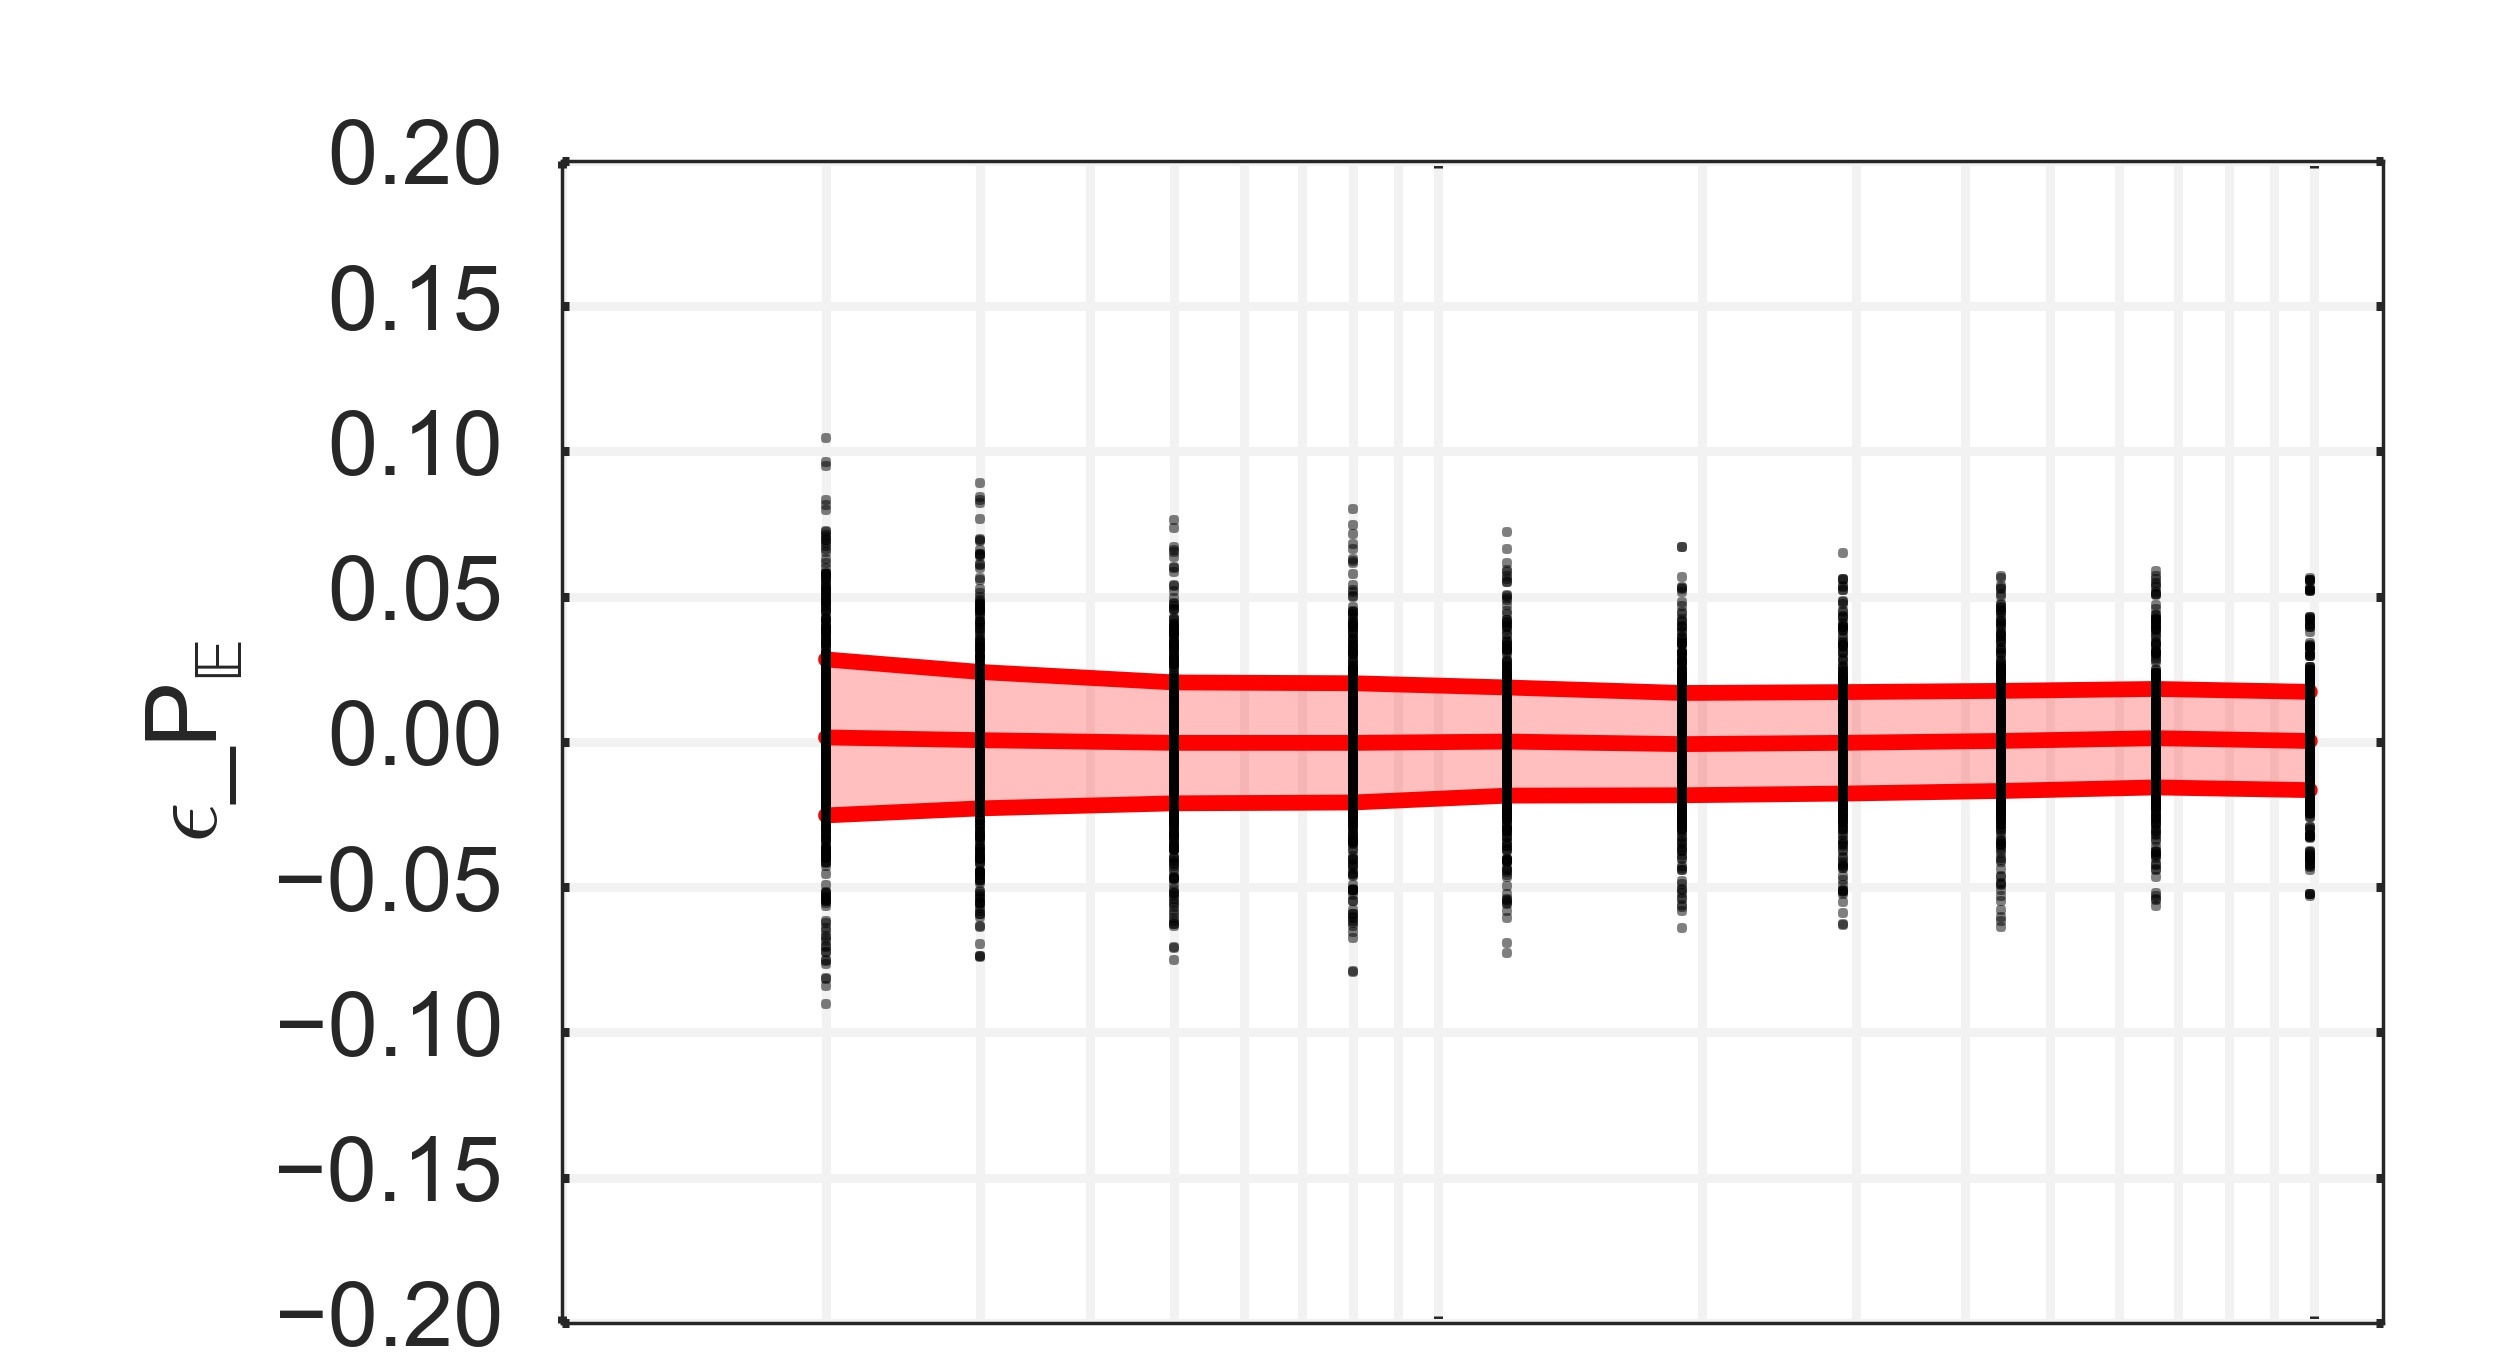
\includegraphics[width=0.3\columnwidth]{Figures/Convergence/CV_E_P.pdf}
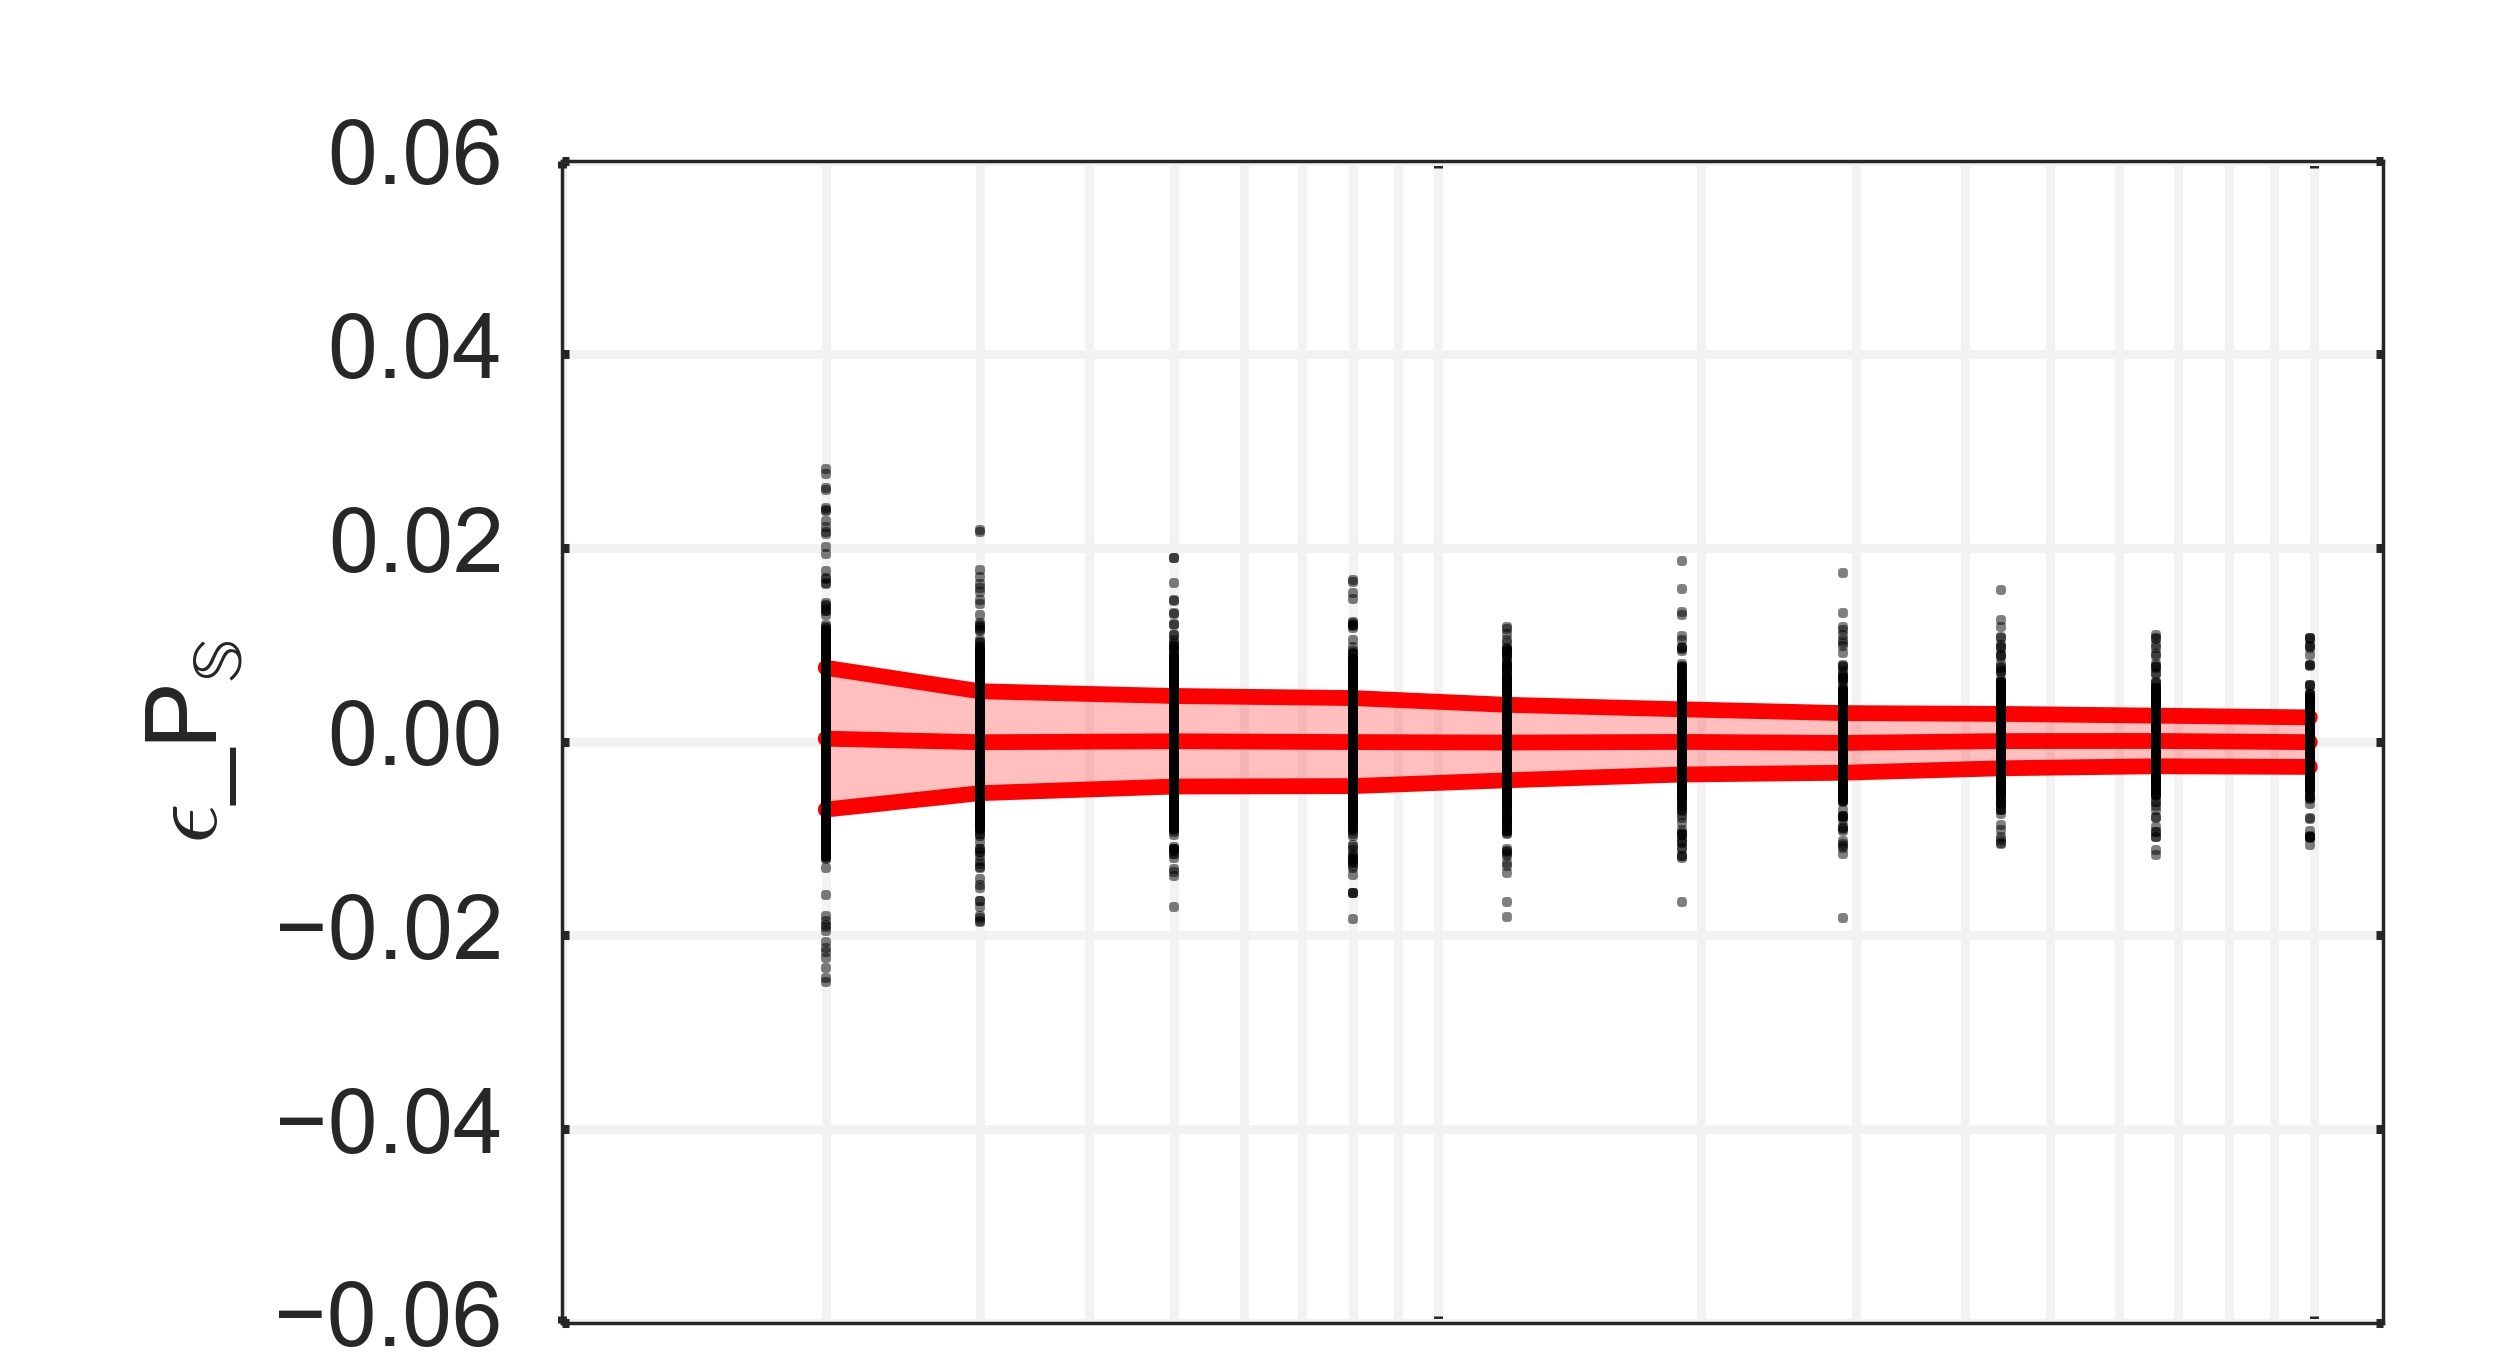
\includegraphics[width=0.3\columnwidth]{Figures/Convergence/CV_V_P.pdf}
\includegraphics[width=0.3\columnwidth]{Figures/Convergence/CV_A_P.pdf}
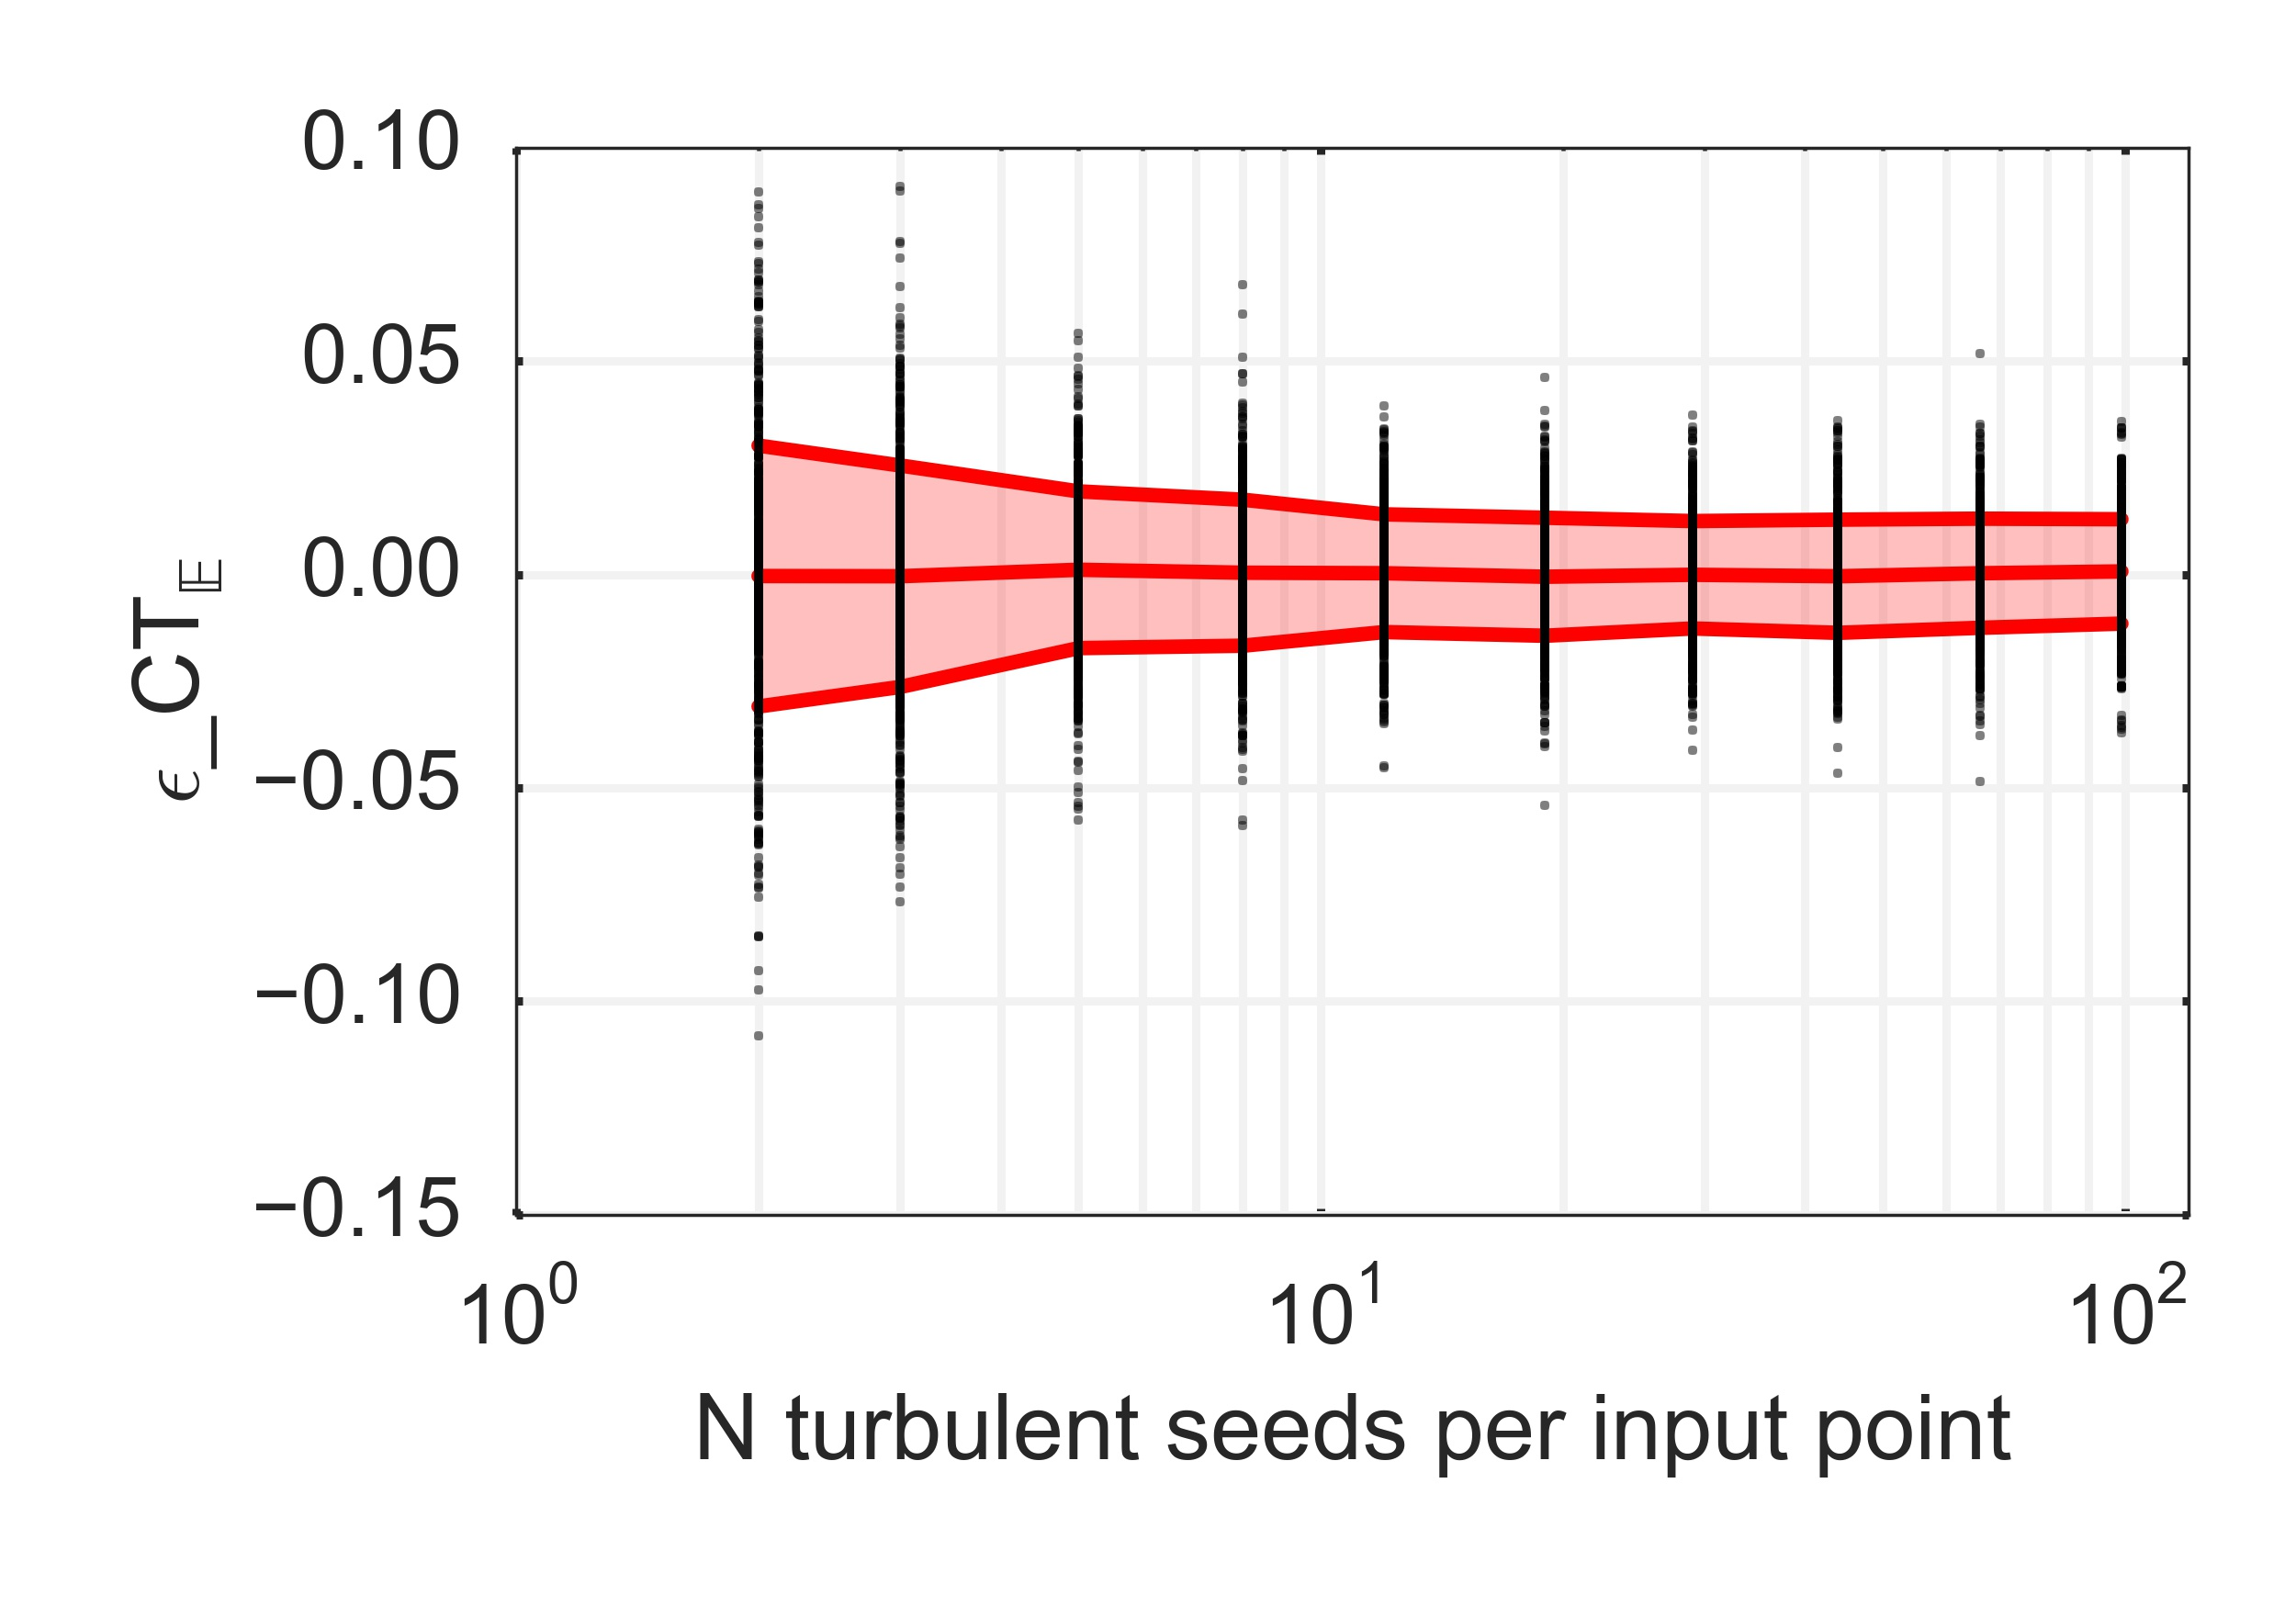
\includegraphics[width=0.3\columnwidth]{Figures/Convergence/CV_E_CT.pdf}
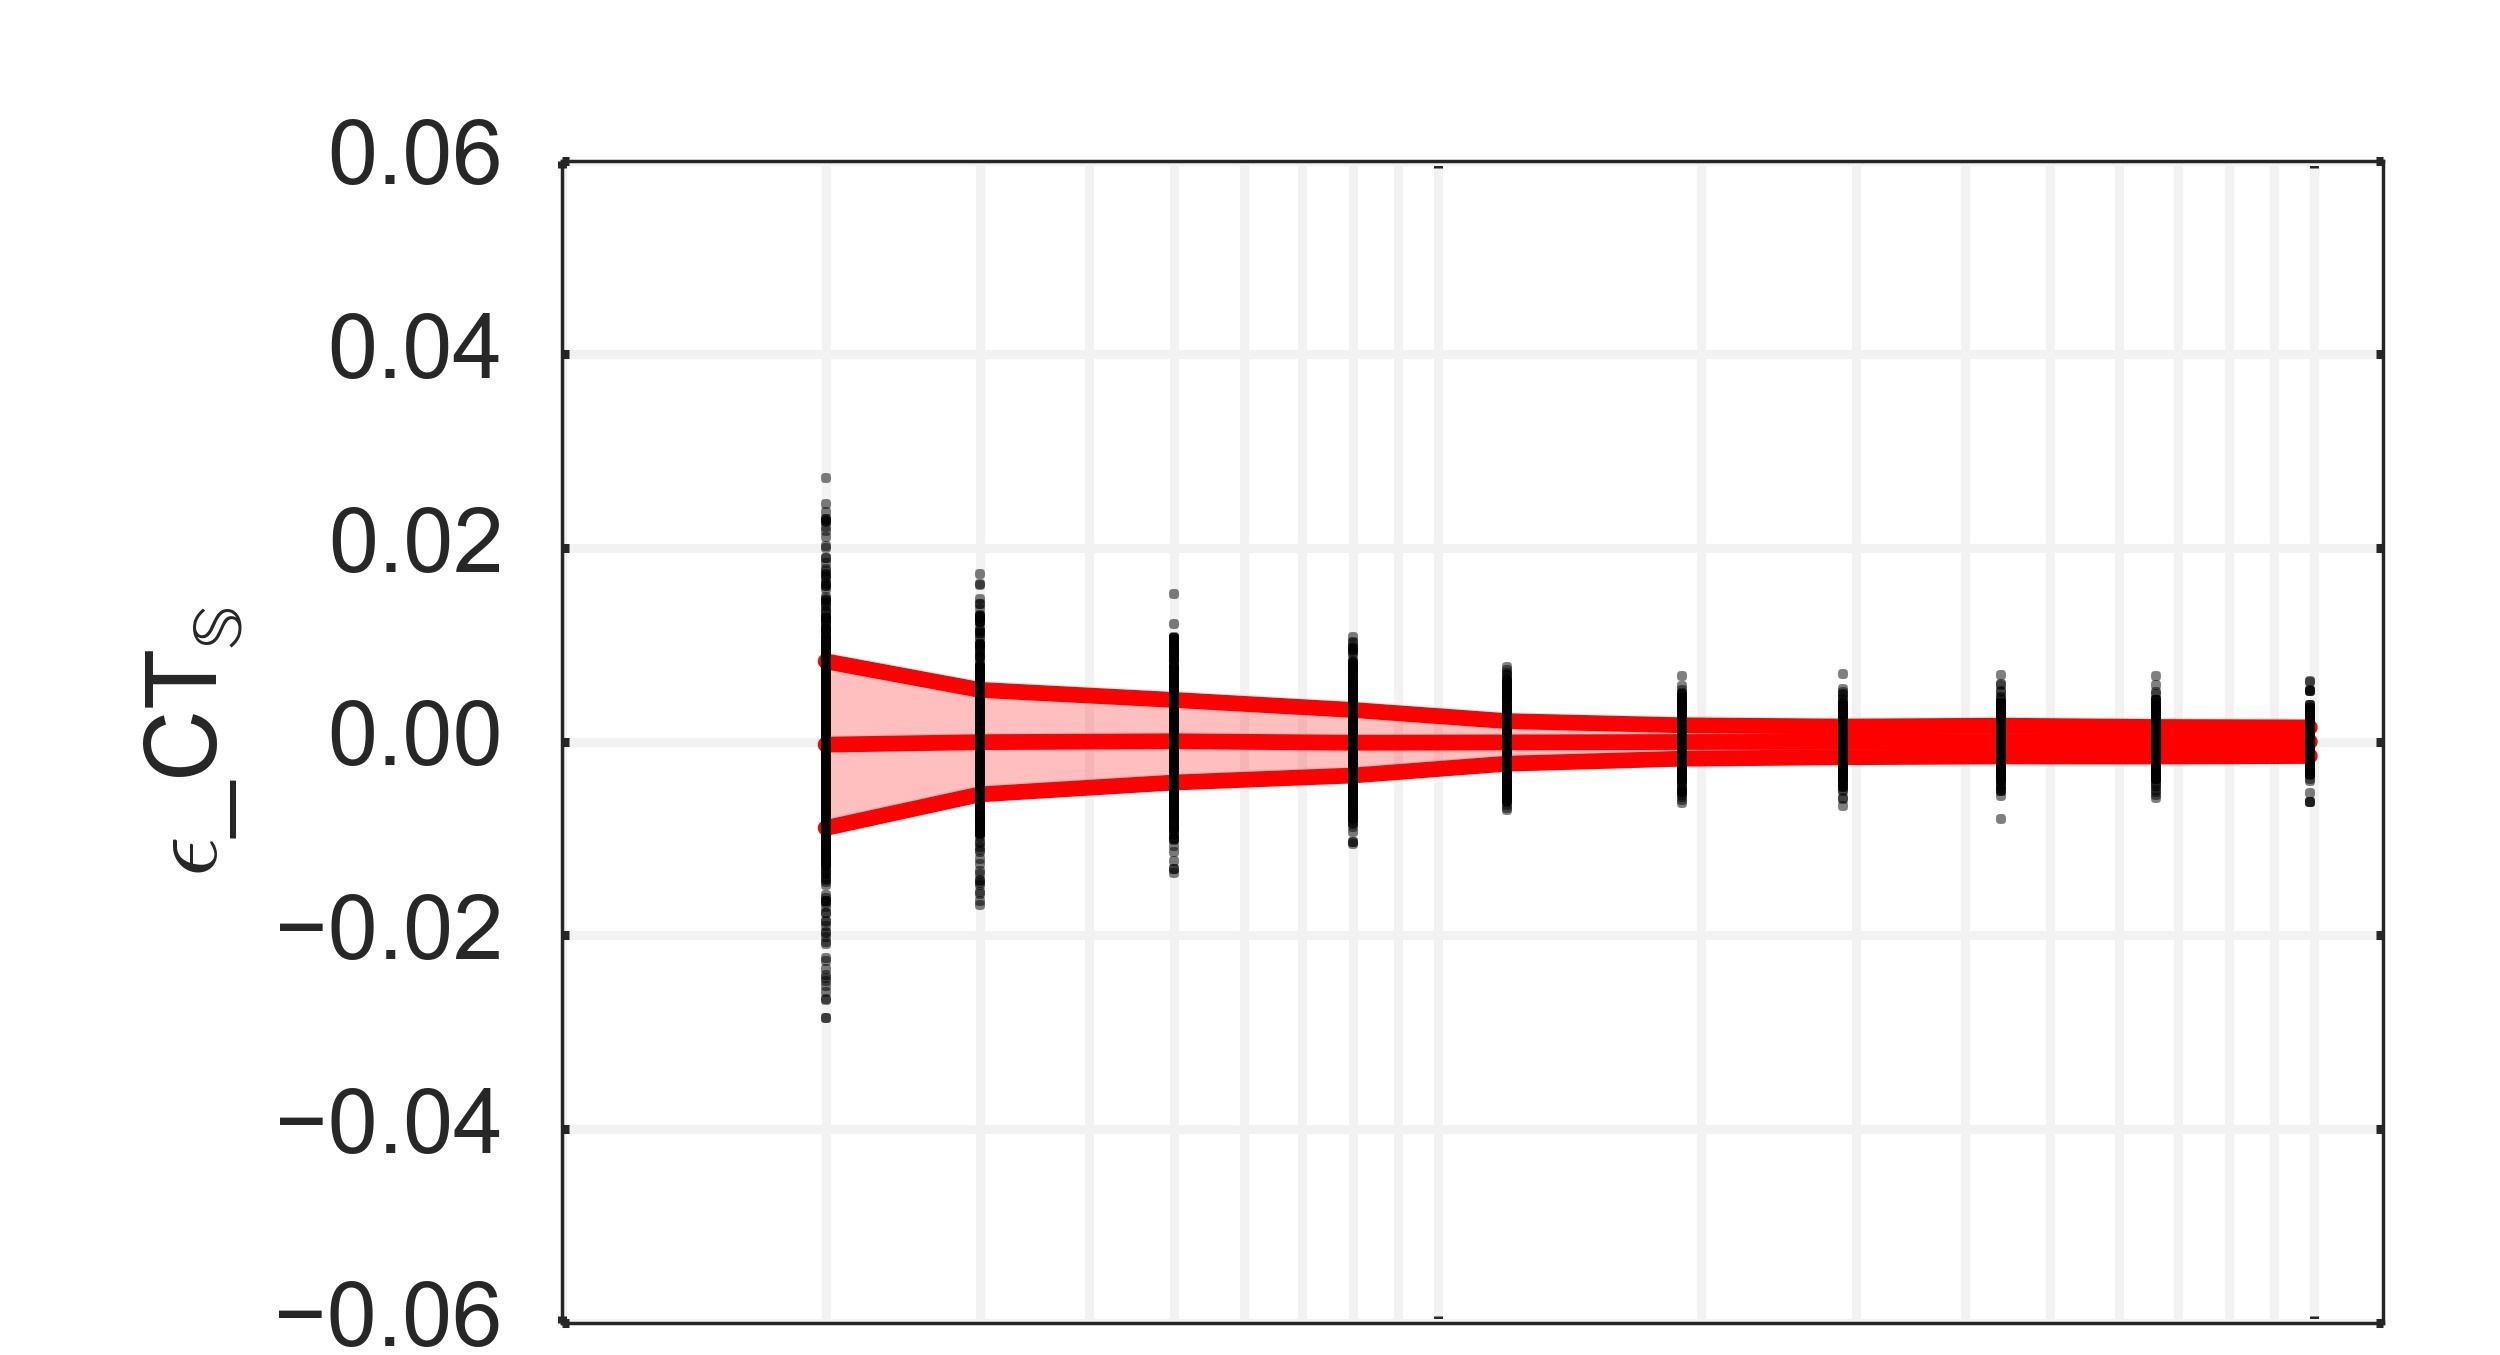
\includegraphics[width=0.3\columnwidth]{Figures/Convergence/CV_V_CT.pdf}
\includegraphics[width=0.3\columnwidth]{Figures/Convergence/CV_A_CT.pdf}
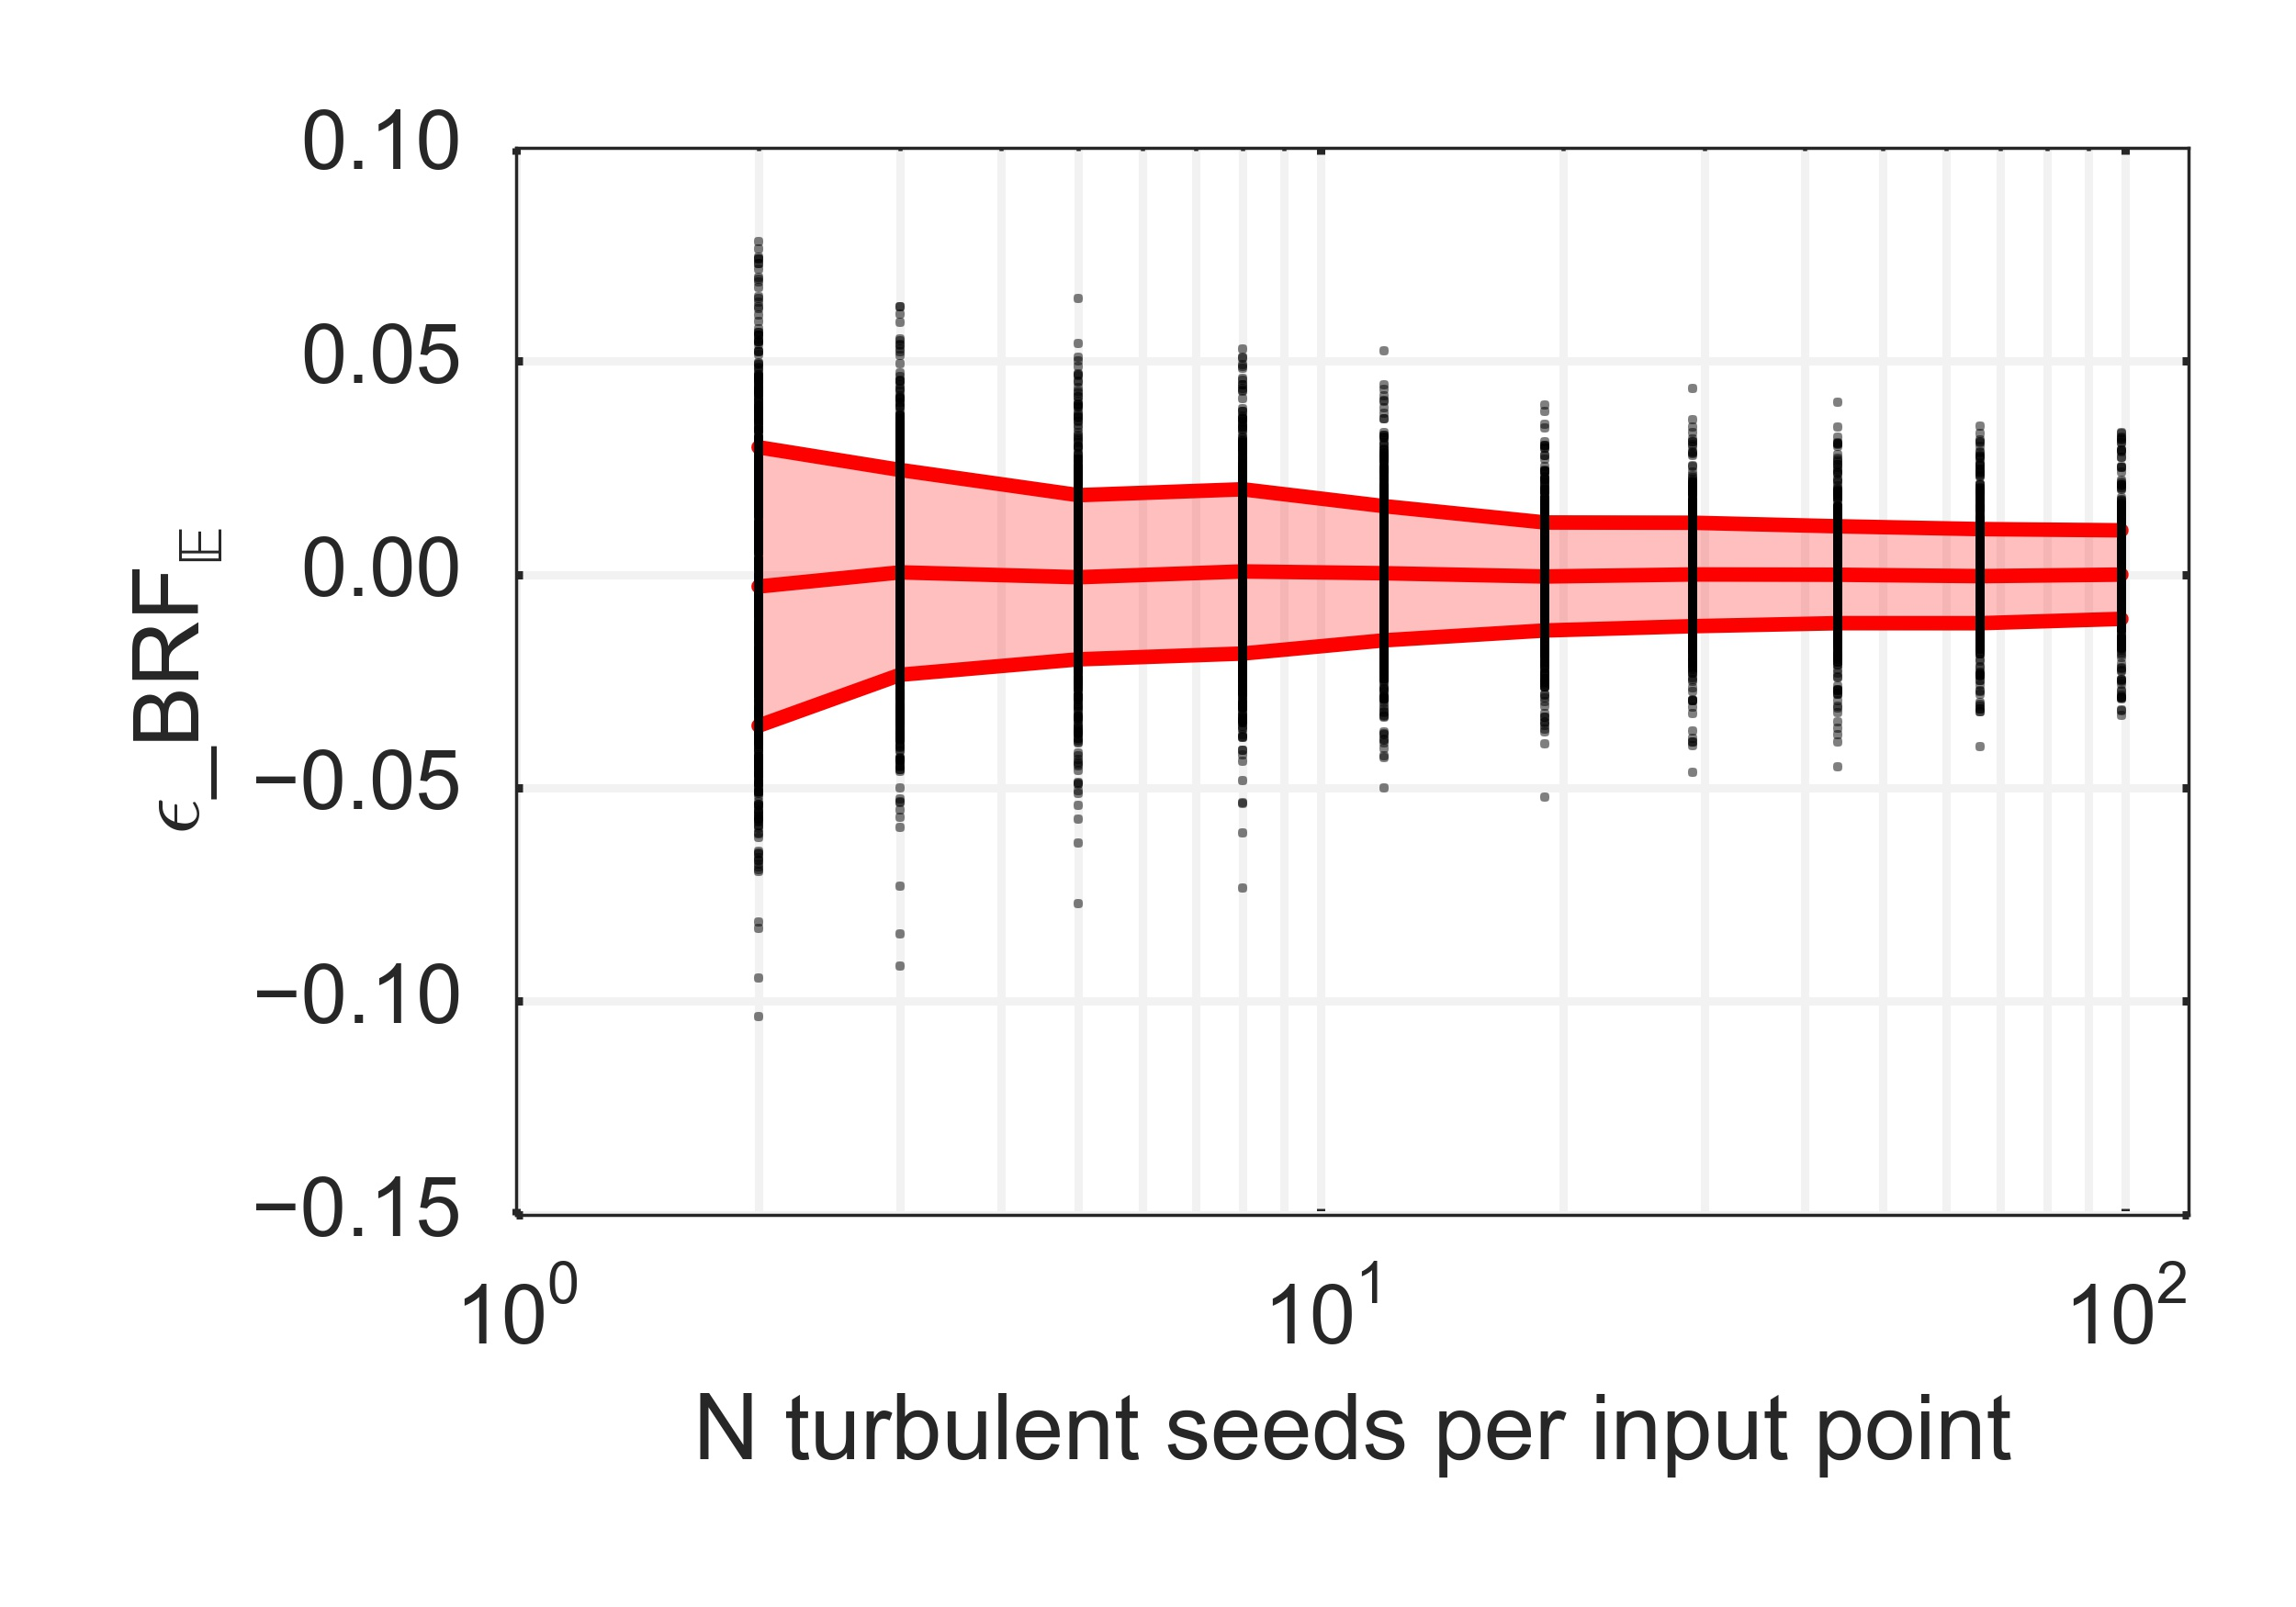
\includegraphics[width=0.3\columnwidth]{Figures/Convergence/CV_E_BRFBM_EFL_M12.pdf}
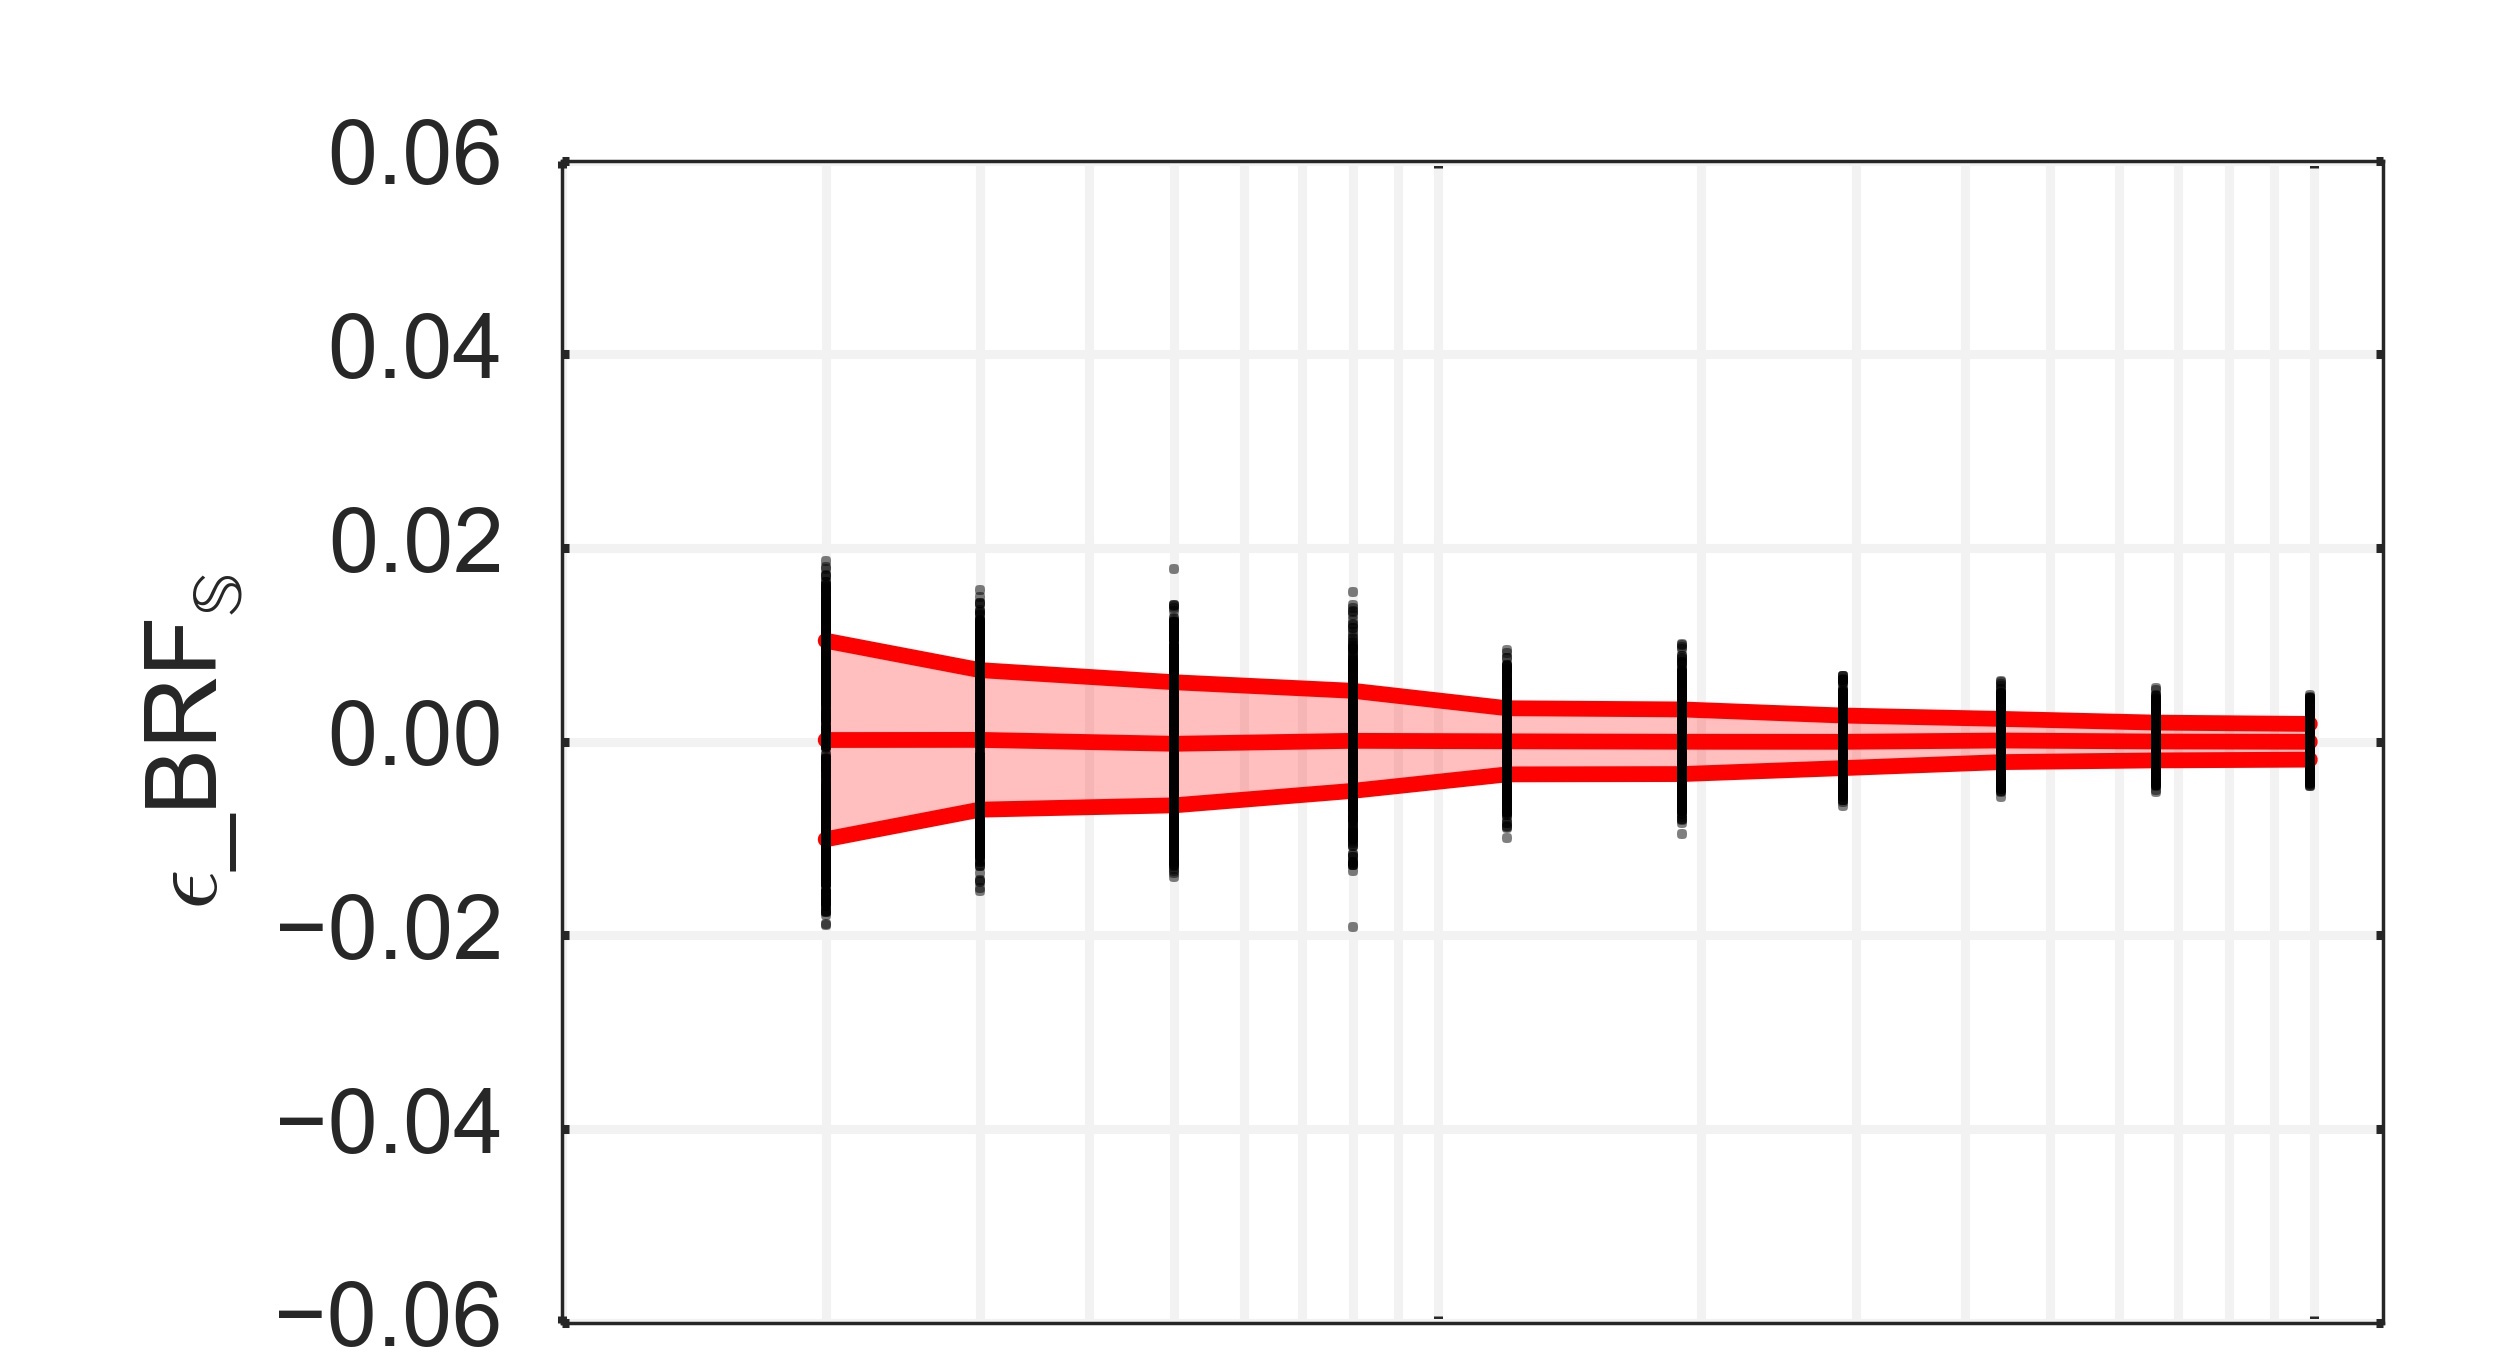
\includegraphics[width=0.3\columnwidth]{Figures/Convergence/CV_V_BRFBM_EFL_M12.pdf}
\includegraphics[width=0.3\columnwidth]{Figures/Convergence/CV_A_BRFBM_EFL_M12.pdf}
\caption{Convergence of the cross-validation metrics as a function of the number of turbulent seeds per input point. (Black points) Outliers outside the interval [Q1-1.5 IQR, Q3+1.5 IQR]. Where each box plot shows the Q1 (0.25 quantile), median (0.5 quantile), Q3 (0.75 quantile), Q1-1.5 IQR, and Q3+1.5 IQR; where the inter quartile range is IQR=Q3-Q1.}
\label{fig_convergence}
\end{centering}
\end{figure}

\section{Discussion}


The presented approach is a promising replacement of the traditional techniques to explore the global behavior of an aeroelastic model in multiple dimensions. For the DTU 10 MW RWT case (4 dimensional case) it is enough to run 140 input cases (with multiple turbulent inflow realizations), while traditional approaches require in the order of $20^4$ gridsearch/interpolation (full factorial design with  20 points per dimensions) and $10^5-10^6$ variance reduction Monte-Carlo sample \cite{dimitrov2015model}. Furthermore, the present approach enables to build an uncertainty model around the performance of the model to include turbulent inflow realization.

The combined PCE surrogate approach can be used to improve traditional conservative designs in which a worst case scenario for shear and turbulence intensity is considered. The improvement can be to perform reliability based designs, in which the probability of failure can be estimated and with the advantage of having better control of the effect of the safety factors used.

The present approach can also be used to improve the estimation of the annual energy production and of the lifetime equivalent fatigue load based on site specific characteristics. The combined PCE surrogates can be understood as an extension of the power curve. The final PCE is an uncertainty model that predicts the performance of the turbine as a probability distribution for a given inflow condition. This uncertainty model of turbine performance can be easily implemented in the work flow of two applications: (1) An uncertainty quantification of the energy production inside a wind farm problem. (2) A robust wind farm layout optimization problem based on AEP and EFL and their corresponding uncertainties.

To obtain the $\pdf(P)$ and $\pdf(EFL)$ is useful as they can be used for uncertainty estimation of the levelized cost of energy on a yearly basis. The surrogates can be evaluated on a long time series of the local wind resources (in multiple variables) such as the ones predicted by wind resource forecast (WRF) models without considerable extra computational effort. The power surrogate can then predict the inter year variation of energy production while the EFL can be used to estimate the operation and maintenance costs. Such a probabilistic output can be considered to be the input for a decision making tool since the decisions can be taken using a combination of the probability of not succeeding in a wind project (losing money) and the expected losses in the region of failure.

\section{Conclusions}

The present article present a methodology to implement PCE on aeroelastic wind turbine models. PCE are widely use in the uncertainty quantification field due to their efficiency to compute the statistical properties of the output and because the sensitivity analysis is obtained without any additional effort. The main two limitations in the use of PCE for wind energy are: (1) The input distribution of atmospheric parameters are usually jointly distributed with several layers of dependency (2) Some of the output have discontinuities and/or are restricted to certain values (e.g. only positive). The present article has shown how to solve this two problems: the implementation of an iso-probabilistic transformation to de-correlate the inputs, and  the use of a logistic transformation to implement restrictions on the outputs.

The results presented in this article show that there are several inter dependencies between the input variables and between inputs and outputs. Such complicated inter dependencies are very difficult to capture when applying other methods such as interpolation or Gaussian processes. The PCE are ideal for this sort of problem because of the transformation into the uncorrelated space. Additionally, the correlations of between the outputs are fully captured when using PCE. This occurs because each of the outputs has a dependency on the inputs: the correlation between the outputs is capture by the dependency in the inputs. In the extra material for this article you can find the full pair plot (4 inputs and 7 outputs) of the training dataset and the resulting surrogate.

The final results shows a promising new approach to communicate the performance of a wind turbine between the turbine manufacturers and the project operators. It is common practice in the wind energy industry to not share the aeroelastic information of a wind turbine. Because of that, the wind project planners and operators do not have enough information about the expected performance of a turbine at the site they are developing, on top of this, there is no model for the uncertainty of the turbine performance. We propose that the multiple PCE should be fitted by the manufacturer and then, the PCe can be shared with all their users and clients. In this way, the turbine manufacturers can keep the information about their turbine and controller design classified. By receiving the PCE of the wind turbine performance the developers will be able to perform uncertainty estimations on their projects which will lead to a better estimation of the AEP and the uncertainty in AEP. As an additional benefit, the project developers will obtain the information about the fatigue damage of the turbine, which can lead to wind plant optimization that considers the damage that the turbines experiences through the years of operation. Fatigue information can lead to better operation and maintenance models which will improve the over all estimation of levelized cost of energy and of its uncertainty.

\section{Acknowledgments}

This work was supported by the International Collaborative Energy Technology R\&D Program of the Korea Institute of Energy Technology Evaluation and Planning (KETEP), granted financial resource from the Ministry of Trade, Industry \& Energy, Republic of Korea. (No. 20138520021140).


%% The Appendices part is started with the command \appendix;
%% appendix sections are then done as normal sections
%% \appendix

%% \section{}
%% \label{}

%% If you have bibdatabase file and want bibtex to generate the
%% bibitems, please use
\section*{References}
\tiny
\bibliographystyle{elsarticle-num}
\bibliography{bib}

%% else use the following coding to input the bibitems directly in the
%% TeX file.

\begin{thebibliography}{00}

%% \bibitem{label}
%% Text of bibliographic item
%% \bibitem{}

\end{thebibliography}

\section*{Appendix A: Polynomial coefficients}
\small
The resulting polynomial surrogates for the DTU 10 MW RWT are presented in this section. Note that in order to use them it is required to have the Rosenblatt transformation ($R$) and the Logistic transformation ($L$). Additionally, the multi-indexes are given for the Legendre polynomials on each dimension of $\vw$ with their correspondent coefficient.

$$y_k = \frac{L^{-1}(\hat{z}_k(R^{-1}(\vx))) - a_k}{k_k}$$

\tiny

\begin{table}[h!]
\begin{minipage}[h!]{0.23\textwidth}
\resizebox{0.9\linewidth}{!}{
\begin{tabular}{|c|ccccc|}
\hline
$j$ &  $l_0$ &  $l_1$ &  $l_2$ &  $l_3$ &  $c_j$ \\
\hline
0  &   1 &   0 &   0 &   0 &   17.658188 \\
1  &   2 &   0 &   0 &   0 &  -77.457857 \\
2  &   3 &   0 &   0 &   0 &  216.397012 \\
3  &   4 &   0 &   0 &   0 & -240.828255 \\
4  &   5 &   0 &   0 &   0 &   90.264172 \\
5  &   3 &   1 &   0 &   0 &    2.033018 \\
6  &   0 &   1 &   0 &   0 &   -0.202756 \\
7  &   1 &   1 &   0 &   0 &    0.605953 \\
8  &   2 &   1 &   0 &   0 &   -2.672805 \\
9  &   1 &   2 &   0 &   0 &   -0.068018 \\
10 &   0 &   2 &   0 &   0 &    0.351076 \\
11 &   0 &   3 &   0 &   0 &   -0.162741 \\
12 &   1 &   0 &   1 &   0 &    0.075779 \\
13 &   2 &   0 &   1 &   0 &    0.387081 \\
14 &   0 &   1 &   1 &   0 &    0.351949 \\
15 &   0 &   2 &   1 &   0 &   -0.550565 \\
16 &   0 &   3 &   1 &   0 &    0.367043 \\
17 &   0 &   0 &   1 &   0 &   -0.925248 \\
18 &   1 &   0 &   2 &   0 &   -0.393105 \\
19 &   0 &   1 &   2 &   0 &    0.095203 \\
20 &   0 &   0 &   2 &   0 &    1.013455 \\
21 &   0 &   0 &   3 &   0 &   -0.352174 \\
22 &   1 &   0 &   0 &   1 &   -0.116624 \\
23 &   2 &   0 &   0 &   1 &    0.059727 \\
24 &   1 &   1 &   0 &   1 &    0.114842 \\
25 &   0 &   1 &   0 &   1 &    0.655366 \\
26 &   0 &   2 &   0 &   1 &   -0.145911 \\
27 &   0 &   0 &   1 &   1 &    1.989207 \\
28 &   1 &   0 &   1 &   1 &   -0.033820 \\
29 &   2 &   0 &   1 &   1 &   -0.212130 \\
30 &   0 &   1 &   1 &   1 &   -0.419338 \\
31 &   0 &   0 &   2 &   1 &   -1.992542 \\
32 &   0 &   0 &   3 &   1 &    0.138458 \\
33 &   0 &   0 &   0 &   1 &   -0.456983 \\
34 &   1 &   0 &   2 &   1 &    0.367355 \\
35 &   0 &   1 &   0 &   2 &   -0.737762 \\
36 &   0 &   0 &   1 &   2 &   -1.414890 \\
37 &   0 &   0 &   0 &   2 &    0.395138 \\
38 &   0 &   0 &   2 &   2 &    1.776157 \\
39 &   0 &   1 &   0 &   3 &    0.483475 \\
40 &   0 &   0 &   1 &   3 &   -0.341771 \\
41 &   0 &   0 &   0 &   0 &   -3.032346 \\
42 &   0 &   0 &   0 &   3 &   -0.079862 \\
\hline
\end{tabular}}
\caption{\tiny P\_E PCE.}
\end{minipage}%
%
\begin{minipage}[h!]{0.23\textwidth}
\resizebox{0.9\linewidth}{!}{
\begin{tabular}{|c|ccccc|}
\hline
$j$ &  $l_0$ &  $l_1$ &  $l_2$ &  $l_3$ &  $c_j$ \\
\hline
0  &   1 &   0 &   0 &   0 &   21.273245 \\
1  &   2 &   0 &   0 &   0 & -143.486636 \\
2  &   3 &   0 &   0 &   0 &  482.039548 \\
3  &   4 &   0 &   0 &   0 & -684.736104 \\
4  &   5 &   0 &   0 &   0 &  320.084412 \\
5  &   1 &   1 &   0 &   0 &   -3.744185 \\
6  &   3 &   1 &   0 &   0 &   56.599143 \\
7  &   4 &   1 &   0 &   0 &  -38.008942 \\
8  &   0 &   1 &   0 &   0 &    5.160127 \\
9  &   2 &   1 &   0 &   0 &  -21.023263 \\
10 &   1 &   2 &   0 &   0 &   14.580231 \\
11 &   0 &   2 &   0 &   0 &  -11.101796 \\
12 &   0 &   3 &   0 &   0 &    7.627074 \\
13 &   1 &   3 &   0 &   0 &   -9.547355 \\
14 &   1 &   0 &   1 &   0 &    4.893289 \\
15 &   2 &   0 &   1 &   0 &    3.838437 \\
16 &   3 &   0 &   1 &   0 &   -2.711066 \\
17 &   1 &   1 &   1 &   0 &   -2.494926 \\
18 &   0 &   1 &   1 &   0 &   -6.846142 \\
19 &   2 &   1 &   1 &   0 &    0.379806 \\
20 &   0 &   2 &   1 &   0 &    6.995239 \\
21 &   0 &   3 &   1 &   0 &   -5.778094 \\
22 &   0 &   0 &   1 &   0 &    0.814946 \\
23 &   1 &   0 &   2 &   0 &   -1.199063 \\
24 &   0 &   1 &   2 &   0 &    3.839858 \\
25 &   0 &   2 &   2 &   0 &    1.671901 \\
26 &   0 &   0 &   2 &   0 &   -0.354253 \\
27 &   1 &   0 &   3 &   0 &   -5.277999 \\
28 &   0 &   0 &   3 &   0 &    0.678668 \\
29 &   0 &   1 &   3 &   0 &   -0.792169 \\
30 &   1 &   0 &   0 &   1 &    2.198590 \\
31 &   1 &   1 &   0 &   1 &   -4.886437 \\
32 &   0 &   2 &   0 &   1 &    0.138720 \\
33 &   1 &   2 &   0 &   1 &   -0.277441 \\
34 &   1 &   1 &   1 &   1 &    6.950392 \\
35 &   0 &   0 &   1 &   1 &   -3.899184 \\
36 &   1 &   0 &   1 &   1 &  -19.451206 \\
37 &   0 &   1 &   1 &   1 &    9.447948 \\
38 &   0 &   0 &   2 &   1 &   -2.490608 \\
39 &   0 &   0 &   0 &   1 &   -0.270775 \\
40 &   0 &   1 &   0 &   1 &    5.679932 \\
41 &   1 &   0 &   2 &   1 &   17.562152 \\
42 &   0 &   1 &   2 &   1 &   -5.602658 \\
43 &   1 &   0 &   0 &   2 &    1.968783 \\
44 &   1 &   1 &   0 &   2 &    1.688681 \\
45 &   0 &   1 &   1 &   2 &   -6.431774 \\
46 &   0 &   0 &   1 &   2 &   12.623057 \\
47 &   0 &   0 &   0 &   2 &    0.917524 \\
48 &   0 &   1 &   0 &   3 &   13.051221 \\
49 &   0 &   0 &   1 &   3 &   -5.873527 \\
50 &   0 &   0 &   0 &   0 &   -4.625465 \\
51 &   0 &   1 &   0 &   2 &  -17.205286 \\
52 &   0 &   0 &   0 &   3 &   -1.027379 \\
53 &   0 &   0 &   0 &   4 &   -0.926286 \\
\hline
\end{tabular}}
\caption{\tiny P\_S PCE.}
\end{minipage}%
%
\begin{minipage}[h!]{0.23\textwidth}
\resizebox{0.9\linewidth}{!}{
\begin{tabular}{|c|ccccc|}
\hline
$j$ &  $l_0$ &  $l_1$ &  $l_2$ &  $l_3$ &  $c_j$ \\
\hline
0   &   4 &   0 &   0 &   0 & -827.257448 \\
1   &   5 &   0 &   0 &   0 &  800.815720 \\
2   &   6 &   0 &   0 &   0 & -280.606232 \\
3   &   3 &   1 &   0 &   0 &   17.004492 \\
4   &   4 &   1 &   0 &   0 &   -8.862149 \\
5   &   5 &   1 &   0 &   0 &   -0.515021 \\
6   &   0 &   1 &   0 &   0 &   -2.597773 \\
7   &   0 &   2 &   0 &   0 &    6.136855 \\
8   &   0 &   3 &   0 &   0 &   -2.144046 \\
9   &   0 &   4 &   0 &   0 &   -6.041061 \\
10  &   1 &   4 &   0 &   0 &   -2.793737 \\
11  &   0 &   5 &   0 &   0 &    4.207707 \\
12  &   1 &   0 &   1 &   0 &    2.004547 \\
13  &   2 &   0 &   1 &   0 &    2.484504 \\
14  &   3 &   0 &   1 &   0 &    2.370726 \\
15  &   1 &   1 &   1 &   0 &  -10.335456 \\
16  &   2 &   1 &   1 &   0 &    3.463070 \\
17  &   1 &   2 &   1 &   0 &    5.221005 \\
18  &   2 &   2 &   1 &   0 &   -0.066848 \\
19  &   1 &   3 &   1 &   0 &   -1.741936 \\
20  &   3 &   1 &   2 &   0 &   -0.662732 \\
21  &   0 &   1 &   2 &   0 &  -15.091321 \\
22  &   0 &   2 &   2 &   0 &   10.824525 \\
23  &   0 &   3 &   2 &   0 &   -3.766392 \\
24  &   0 &   0 &   2 &   0 &    9.992672 \\
25  &   1 &   0 &   3 &   0 &    2.168159 \\
26  &   1 &   1 &   3 &   0 &   -4.415429 \\
27  &   0 &   0 &   4 &   0 &    4.140158 \\
28  &   2 &   0 &   0 &   1 &   -4.118752 \\
29  &   3 &   0 &   0 &   1 &    3.556601 \\
30  &   1 &   1 &   0 &   1 &   -3.060339 \\
31  &   2 &   1 &   0 &   1 &    1.941121 \\
32  &   0 &   2 &   0 &   1 &  -15.283344 \\
33  &   0 &   2 &   1 &   1 &    7.305088 \\
34  &   0 &   0 &   1 &   1 &    5.102290 \\
35  &   0 &   3 &   1 &   1 &   -2.128947 \\
36  &   1 &   1 &   2 &   1 &   -0.400943 \\
37  &   0 &   2 &   2 &   1 &   -4.559060 \\
38  &   0 &   0 &   2 &   1 &  -15.287274 \\
39  &   0 &   0 &   4 &   1 &   -7.996038 \\
40  &   0 &   0 &   0 &   1 &    0.502381 \\
41  &   0 &   0 &   3 &   1 &   17.420762 \\
42  &   1 &   0 &   0 &   2 &    6.903704 \\
43  &   2 &   0 &   0 &   2 &   -0.622189 \\
44  &   1 &   1 &   0 &   2 &   -1.851140 \\
45  &   2 &   1 &   0 &   2 &   -1.872743 \\
46  &   0 &   1 &   1 &   2 &   -1.905920 \\
47  &   0 &   0 &   1 &   2 &   -0.501649 \\
48  &   0 &   0 &   2 &   2 &    1.701844 \\
49  &   2 &   0 &   0 &   3 &    1.505283 \\
50  &   1 &   1 &   0 &   3 &    2.638588 \\
51  &   0 &   1 &   0 &   3 &   -2.933920 \\
52  &   1 &   0 &   1 &   3 &    0.909555 \\
53  &   0 &   0 &   0 &   4 &   -2.607652 \\
54  &   0 &   0 &   0 &   0 &    1.886055 \\
55  &   1 &   0 &   0 &   0 &   -0.923786
\end{tabular}}
\end{minipage}%
%
\begin{minipage}[h!]{0.23\textwidth}
\resizebox{0.9\linewidth}{!}{
\begin{tabular}{|c|ccccc|}
\hline
$j$ &  $l_0$ &  $l_1$ &  $l_2$ &  $l_3$ &  $c_j$ \\
\hline
56  &   2 &   0 &   0 &   0 &  -57.123284 \\
57  &   3 &   0 &   0 &   0 &  360.129037 \\
58  &   1 &   1 &   0 &   0 &    6.551412 \\
59  &   2 &   1 &   0 &   0 &  -13.178827 \\
60  &   1 &   2 &   0 &   0 &  -10.882394 \\
61  &   2 &   2 &   0 &   0 &    3.012151 \\
62  &   3 &   2 &   0 &   0 &    2.228364 \\
63  &   1 &   3 &   0 &   0 &   11.486608 \\
64  &   2 &   3 &   0 &   0 &   -4.152913 \\
65  &   4 &   0 &   1 &   0 &   -5.319179 \\
66  &   3 &   1 &   1 &   0 &    0.662732 \\
67  &   0 &   1 &   1 &   0 &    8.984505 \\
68  &   0 &   2 &   1 &   0 &   -9.350190 \\
69  &   0 &   3 &   1 &   0 &    3.926594 \\
70  &   0 &   0 &   1 &   0 &   -3.893998 \\
71  &   1 &   0 &   2 &   0 &   -3.635569 \\
72  &   2 &   0 &   2 &   0 &   -6.470444 \\
73  &   3 &   0 &   2 &   0 &    6.374993 \\
74  &   1 &   1 &   2 &   0 &   15.183301 \\
75  &   2 &   1 &   2 &   0 &   -3.865114 \\
76  &   1 &   2 &   2 &   0 &   -3.898113 \\
77  &   0 &   1 &   3 &   0 &    5.761567 \\
78  &   0 &   2 &   3 &   0 &   -1.239554 \\
79  &   0 &   0 &   3 &   0 &  -10.324073 \\
80  &   1 &   0 &   0 &   1 &    0.319789 \\
81  &   4 &   0 &   0 &   1 &   -1.499582 \\
82  &   3 &   1 &   0 &   1 &    0.421050 \\
83  &   0 &   1 &   0 &   1 &    3.787639 \\
84  &   1 &   2 &   0 &   1 &    7.826755 \\
85  &   1 &   3 &   0 &   1 &   -5.966679 \\
86  &   0 &   3 &   0 &   1 &   16.844501 \\
87  &   0 &   4 &   0 &   1 &   -5.764745 \\
88  &   1 &   0 &   1 &   1 &   -2.111665 \\
89  &   1 &   1 &   1 &   1 &   -0.441080 \\
90  &   0 &   1 &   1 &   1 &   -5.536196 \\
91  &   1 &   0 &   2 &   1 &    2.840954 \\
92  &   0 &   1 &   2 &   1 &   10.786568 \\
93  &   0 &   1 &   3 &   1 &   -4.628595 \\
94  &   0 &   1 &   0 &   2 &    3.239449 \\
95  &   1 &   0 &   1 &   2 &    1.621912 \\
96  &   0 &   0 &   0 &   2 &   -4.623801 \\
97  &   0 &   2 &   0 &   2 &   -0.600983 \\
98  &   1 &   0 &   2 &   2 &   -2.640482 \\
99  &   0 &   0 &   0 &   3 &    6.205667 \\
100 &   1 &   0 &   0 &   3 &   -9.102199 \\
101 &   0 &   2 &   0 &   3 &    0.343968 \\
102 &   0 &   0 &   1 &   3 &   -1.377748 \\
103 &   0 &   1 &   1 &   3 &    0.458134 \\
104 &   0 &   0 &   2 &   3 &    0.040432 \\
105 &   1 &   0 &   0 &   4 &    2.802899 \\
106 &   0 &   1 &   0 &   4 &    0.800728 \\
107 &   0 &   0 &   1 &   4 &    0.696161 \\
\hline
\end{tabular}}
\caption{\tiny CT\_E PCE.}
\end{minipage}%
\end{table}
%
\begin{table}
\begin{minipage}[h!]{0.23\textwidth}
\resizebox{0.9\linewidth}{!}{
\begin{tabular}{|c|ccccc|}
\hline
$j$ &  $l_0$ &  $l_1$ &  $l_2$ &  $l_3$ &  $c_j$ \\
\hline
0  &   1 &   0 &   0 &   0 &  -1.588617 \\
1  &   2 &   0 &   0 &   0 &   6.960288 \\
2  &   3 &   0 &   0 &   0 & -13.078366 \\
3  &   4 &   0 &   0 &   0 &   3.658774 \\
4  &   0 &   1 &   0 &   0 &   1.268715 \\
5  &   1 &   1 &   0 &   0 &  -1.307230 \\
6  &   2 &   1 &   0 &   0 &   0.893358 \\
7  &   0 &   2 &   0 &   0 &  -1.584460 \\
8  &   0 &   3 &   0 &   0 &   1.124566 \\
9  &   1 &   0 &   1 &   0 &   0.096560 \\
10 &   0 &   1 &   1 &   0 &   0.570601 \\
11 &   0 &   2 &   1 &   0 &  -0.279196 \\
12 &   0 &   0 &   1 &   0 &  -0.193227 \\
13 &   0 &   1 &   2 &   0 &  -0.003906 \\
14 &   0 &   0 &   2 &   0 &  -0.065941 \\
15 &   1 &   0 &   0 &   1 &   0.015114 \\
16 &   2 &   0 &   0 &   1 &  -0.124400 \\
17 &   0 &   1 &   0 &   1 &   0.231847 \\
18 &   0 &   0 &   1 &   1 &   0.127705 \\
19 &   0 &   1 &   1 &   1 &  -0.575000 \\
20 &   0 &   0 &   2 &   1 &   0.017503 \\
21 &   0 &   0 &   0 &   1 &   0.037185 \\
22 &   1 &   0 &   0 &   2 &   0.172970 \\
23 &   0 &   0 &   1 &   2 &   0.207437 \\
24 &   0 &   0 &   0 &   2 &  -0.249519 \\
25 &   0 &   0 &   0 &   0 &  -1.697421 \\
\hline
\end{tabular}}
\caption{\tiny CT\_S PCE.}
%
\bigskip
%
\resizebox{0.9\linewidth}{!}{
\begin{tabular}{|c|ccccc|}
\hline
$j$ &  $l_0$ &  $l_1$ &  $l_2$ &  $l_3$ &  $c_j$ \\
\hline
0  &   4 &   0 &   0 &   0 &  62.694878 \\
1  &   5 &   0 &   0 &   0 & -62.819279 \\
2  &   6 &   0 &   0 &   0 &  26.414390 \\
3  &   3 &   1 &   0 &   0 &   5.073870 \\
4  &   4 &   1 &   0 &   0 &  -1.010211 \\
5  &   0 &   1 &   0 &   0 &  -1.232956 \\
6  &   0 &   2 &   0 &   0 &   3.032444 \\
7  &   0 &   3 &   0 &   0 &  -1.380097 \\
8  &   0 &   4 &   0 &   0 &  -2.786755 \\
9  &   0 &   5 &   0 &   0 &   2.762271 \\
10 &   1 &   0 &   1 &   0 &   1.593698 \\
11 &   2 &   0 &   1 &   0 &   1.306560 \\
12 &   3 &   0 &   1 &   0 &  -1.289262 \\
13 &   1 &   1 &   1 &   0 &  -1.960311 \\
14 &   2 &   1 &   1 &   0 &   0.462671 \\
15 &   1 &   2 &   1 &   0 &   1.284869 \\
16 &   0 &   1 &   2 &   0 &   2.583334 \\
17 &   0 &   2 &   2 &   0 &   0.429339 \\
18 &   0 &   0 &   2 &   0 &  -0.068526 \\
19 &   1 &   0 &   3 &   0 &  -1.296834 \\
20 &   2 &   0 &   3 &   0 &   1.644857 \\
21 &   1 &   1 &   3 &   0 &   1.386674 \\
22 &   0 &   1 &   4 &   0 &   1.237224 \\
23 &   0 &   0 &   4 &   0 &  -0.374613 \\
24 &   2 &   0 &   0 &   1 &  -6.958940 \\
25 &   3 &   0 &   0 &   1 &   5.302168 \\
26 &   1 &   1 &   0 &   1 &  -0.544489 \\
27 &   2 &   1 &   0 &   1 &  -0.096270 \\
28 &   0 &   2 &   0 &   1 &  -9.320285 \\
29 &   0 &   0 &   1 &   1 &  -1.387413 \\
30 &   1 &   1 &   2 &   1 &   2.055372
\end{tabular}}
\end{minipage}%
%
\begin{minipage}[h!]{0.23\textwidth}
\resizebox{0.9\linewidth}{!}{
\begin{tabular}{|c|ccccc|}
\hline
$j$ &  $l_0$ &  $l_1$ &  $l_2$ &  $l_3$ &  $c_j$ \\
\hline
31 &   0 &   2 &   2 &   1 &   0.274349 \\
32 &   0 &   0 &   2 &   1 &   2.407023 \\
33 &   0 &   0 &   4 &   1 &   1.505527 \\
34 &   0 &   0 &   0 &   1 &  -0.481728 \\
35 &   0 &   2 &   1 &   1 &  -0.274349 \\
36 &   0 &   0 &   3 &   1 &  -3.385077 \\
37 &   1 &   0 &   0 &   2 &  -2.410568 \\
38 &   2 &   0 &   0 &   2 &   5.058386 \\
39 &   3 &   0 &   0 &   2 &  -3.556947 \\
40 &   1 &   1 &   0 &   2 &   0.679389 \\
41 &   0 &   1 &   1 &   2 &  -0.627927 \\
42 &   0 &   0 &   1 &   2 &  -0.107242 \\
43 &   0 &   0 &   2 &   2 &   2.167533 \\
44 &   0 &   1 &   0 &   3 &   3.995469 \\
45 &   1 &   0 &   1 &   3 &   0.335097 \\
46 &   0 &   0 &   0 &   0 &  -1.621127 \\
47 &   1 &   0 &   0 &   0 &  -1.236436 \\
48 &   2 &   0 &   0 &   0 &  16.592903 \\
49 &   3 &   0 &   0 &   0 & -40.158224 \\
50 &   1 &   1 &   0 &   0 &   4.115606 \\
51 &   2 &   1 &   0 &   0 &  -6.819207 \\
52 &   1 &   2 &   0 &   0 &  -2.273269 \\
53 &   2 &   2 &   0 &   0 &   1.655239 \\
54 &   3 &   2 &   0 &   0 &  -0.811717 \\
55 &   1 &   3 &   0 &   0 &   0.445370 \\
56 &   4 &   0 &   1 &   0 &   0.589926 \\
57 &   3 &   1 &   1 &   0 &   0.218822 \\
58 &   0 &   1 &   1 &   0 &   2.121804 \\
59 &   0 &   2 &   1 &   0 &  -7.253108 \\
60 &   0 &   3 &   1 &   0 &   8.743509 \\
61 &   0 &   4 &   1 &   0 &  -4.116381 \\
62 &   0 &   0 &   1 &   0 &  -0.998033 \\
63 &   1 &   0 &   2 &   0 &   1.097308 \\
64 &   2 &   0 &   2 &   0 &  -2.685648 \\
65 &   1 &   1 &   2 &   0 &  -1.639455 \\
66 &   0 &   1 &   3 &   0 &  -3.600087 \\
67 &   0 &   0 &   3 &   0 &   1.081131 \\
68 &   1 &   0 &   0 &   1 &   2.818352 \\
69 &   0 &   1 &   0 &   1 &   4.830761 \\
70 &   1 &   2 &   0 &   1 &   0.135315 \\
71 &   0 &   3 &   0 &   1 &   9.122104 \\
72 &   0 &   4 &   0 &   1 &  -4.121466 \\
73 &   1 &   0 &   1 &   1 &   0.121521 \\
74 &   2 &   0 &   1 &   1 &   0.453509 \\
75 &   1 &   1 &   1 &   1 &  -1.363471 \\
76 &   0 &   1 &   1 &   1 &   2.146573 \\
77 &   1 &   0 &   2 &   1 &  -1.027686 \\
78 &   0 &   1 &   2 &   1 &  -2.642740 \\
79 &   0 &   1 &   3 &   1 &   0.864604 \\
80 &   0 &   1 &   0 &   2 &  -6.806370 \\
81 &   0 &   2 &   0 &   2 &   6.654701 \\
82 &   1 &   0 &   1 &   2 &   0.234386 \\
83 &   0 &   0 &   0 &   2 &   0.156466 \\
84 &   0 &   3 &   0 &   2 &  -0.879173 \\
85 &   0 &   0 &   0 &   3 &   1.039756 \\
86 &   1 &   0 &   0 &   3 &  -0.165016 \\
87 &   0 &   2 &   0 &   3 &  -3.557294 \\
88 &   0 &   0 &   1 &   3 &  -0.112527 \\
89 &   0 &   0 &   2 &   3 &  -1.312607 \\
90 &   0 &   0 &   0 &   4 &  -0.680624 \\
\hline
\end{tabular}}
\caption{\tiny BRFBM\_EFL\_M12\_E PCE.}
\end{minipage}%
%
\begin{minipage}[h!]{0.23\textwidth}
\resizebox{0.9\linewidth}{!}{
\begin{tabular}{|c|ccccc|}
\hline
$j$ &  $l_0$ &  $l_1$ &  $l_2$ &  $l_3$ &  $c_j$ \\
\hline
0  &   1 &   0 &   0 &   0 &  5.228706 \\
1  &   2 &   0 &   0 &   0 & -7.300998 \\
2  &   3 &   0 &   0 &   0 &  3.523426 \\
3  &   0 &   1 &   0 &   0 &  0.892945 \\
4  &   1 &   1 &   0 &   0 & -0.438192 \\
5  &   0 &   2 &   0 &   0 & -0.313025 \\
6  &   0 &   3 &   0 &   0 &  0.186111 \\
7  &   1 &   0 &   1 &   0 &  0.086469 \\
8  &   0 &   0 &   1 &   0 & -0.202612 \\
9  &   0 &   0 &   0 &   1 &  0.094581 \\
10 &   1 &   0 &   0 &   1 & -0.149807 \\
11 &   0 &   0 &   0 &   0 & -2.244177 \\
\hline
\end{tabular}}
\caption{\tiny BRFBM\_EFL\_M12\_S PCE.}
%
\bigskip
%
\resizebox{0.9\linewidth}{!}{
\begin{tabular}{|c|ccccc|}
\hline
$j$ &  $l_0$ &  $l_1$ &  $l_2$ &  $l_3$ &  $c_j$ \\
\hline
0  &   1 &   0 &   0 &   0 &   7.492604 \\
1  &   2 &   0 &   0 &   0 & -30.048707 \\
2  &   3 &   0 &   0 &   0 &  36.485874 \\
3  &   4 &   0 &   0 &   0 & -13.644361 \\
4  &   0 &   1 &   0 &   0 &   2.494525 \\
5  &   1 &   1 &   0 &   0 &  -2.510374 \\
6  &   2 &   1 &   0 &   0 &   1.552327 \\
7  &   1 &   2 &   0 &   0 &  -0.404614 \\
8  &   0 &   2 &   0 &   0 &  -2.573943 \\
9  &   0 &   3 &   0 &   0 &   2.080285 \\
10 &   1 &   0 &   1 &   0 &  -0.000183 \\
11 &   0 &   1 &   1 &   0 &  -0.031200 \\
12 &   1 &   1 &   1 &   0 &   0.062401 \\
13 &   0 &   0 &   1 &   0 &   0.024172 \\
14 &   1 &   0 &   0 &   1 &  -0.007061 \\
15 &   1 &   1 &   0 &   1 &   0.363697 \\
16 &   0 &   1 &   0 &   1 &   0.122950 \\
17 &   0 &   2 &   0 &   1 &  -0.300063 \\
18 &   0 &   0 &   1 &   1 &   0.013684 \\
19 &   0 &   0 &   0 &   1 &  -0.086136 \\
20 &   1 &   0 &   0 &   2 &  -0.066080 \\
21 &   0 &   0 &   0 &   2 &   0.029179 \\
22 &   0 &   0 &   0 &   0 &  -0.720555 \\
\hline
\end{tabular}}
\caption{\tiny TBFBM\_EFL\_M4\_E PCE.}
\end{minipage}%
%
\begin{minipage}[h!]{0.23\textwidth}
\resizebox{0.9\linewidth}{!}{
\begin{tabular}{|c|ccccc|}
\hline
$j$ &  $l_0$ &  $l_1$ &  $l_2$ &  $l_3$ &  $c_j$ \\
\hline
0  &   1 &   0 &   0 &   0 &   3.265241 \\
1  &   2 &   0 &   0 &   0 &  -8.920657 \\
2  &   3 &   0 &   0 &   0 & -17.700217 \\
3  &   4 &   0 &   0 &   0 &  44.803873 \\
4  &   5 &   0 &   0 &   0 & -22.380164 \\
5  &   0 &   1 &   0 &   0 &   1.010208 \\
6  &   1 &   1 &   0 &   0 &  -0.840001 \\
7  &   2 &   1 &   0 &   0 &   0.216462 \\
8  &   1 &   2 &   0 &   0 &   0.010459 \\
9  &   0 &   2 &   0 &   0 &  -1.764214 \\
10 &   0 &   3 &   0 &   0 &   1.537057 \\
11 &   1 &   0 &   1 &   0 &   0.187639 \\
12 &   2 &   0 &   1 &   0 &  -0.218385 \\
13 &   0 &   1 &   1 &   0 &   1.742232 \\
14 &   1 &   1 &   1 &   0 &  -0.032924 \\
15 &   0 &   2 &   1 &   0 &  -1.036063 \\
16 &   0 &   0 &   1 &   0 &  -0.158630 \\
17 &   1 &   0 &   2 &   0 &   0.063194 \\
18 &   0 &   1 &   2 &   0 &  -0.290302 \\
19 &   0 &   0 &   2 &   0 &  -0.311188 \\
20 &   0 &   0 &   3 &   0 &   0.012734 \\
21 &   1 &   0 &   0 &   1 &  -0.721490 \\
22 &   2 &   0 &   0 &   1 &   1.069445 \\
23 &   3 &   0 &   0 &   1 &  -0.471808 \\
24 &   1 &   1 &   0 &   1 &   0.701628 \\
25 &   2 &   1 &   0 &   1 &  -0.432925 \\
26 &   0 &   1 &   0 &   1 &   1.772737 \\
27 &   0 &   2 &   0 &   1 &  -0.906239 \\
28 &   0 &   0 &   1 &   1 &   0.394469 \\
29 &   0 &   1 &   1 &   1 &  -4.783365 \\
30 &   0 &   0 &   2 &   1 &   1.489605 \\
31 &   0 &   1 &   2 &   1 &   1.288322 \\
32 &   0 &   0 &   3 &   1 &  -0.484483 \\
33 &   0 &   0 &   0 &   1 &  -0.529695 \\
34 &   0 &   2 &   1 &   1 &   1.787082 \\
35 &   0 &   1 &   0 &   2 &  -0.623935 \\
36 &   0 &   1 &   1 &   2 &   1.362023 \\
37 &   0 &   0 &   1 &   2 &  -0.495626 \\
38 &   0 &   0 &   0 &   2 &   0.592109 \\
39 &   0 &   0 &   2 &   2 &  -0.893638 \\
40 &   0 &   0 &   1 &   3 &   0.488628 \\
41 &   0 &   0 &   0 &   3 &  -0.174881 \\
42 &   0 &   0 &   0 &   4 &  -0.196241 \\
43 &   0 &   0 &   0 &   0 &  -1.328826 \\
\hline
\end{tabular}}
\caption{\tiny TBFBM\_EFL\_M4\_S PCE.}
\end{minipage}%
\end{table}
%
\begin{table}
\begin{minipage}[h!]{0.23\textwidth}
\resizebox{0.9\linewidth}{!}{
\begin{tabular}{|c|ccccc|}
\hline
$j$ &  $l_0$ &  $l_1$ &  $l_2$ &  $l_3$ &  $c_j$ \\
\hline
0  &   1 &   0 &   0 &   0 &   17.697877 \\
1  &   2 &   0 &   0 &   0 &  -78.280278 \\
2  &   3 &   0 &   0 &   0 &  103.037368 \\
3  &   4 &   0 &   0 &   0 &  -41.671488 \\
4  &   1 &   1 &   0 &   0 &   -2.089860 \\
5  &   2 &   1 &   0 &   0 &    1.038843 \\
6  &   0 &   1 &   0 &   0 &    2.316537 \\
7  &   0 &   2 &   0 &   0 &   -2.265180 \\
8  &   0 &   3 &   0 &   0 &    1.561479 \\
9  &   1 &   0 &   1 &   0 &    0.774492 \\
10 &   2 &   0 &   1 &   0 &   -0.476546 \\
11 &   0 &   0 &   1 &   0 &   -0.261296 \\
12 &   0 &   0 &   2 &   0 &   -0.055217 \\
13 &   1 &   0 &   0 &   1 &   -0.118863 \\
14 &   1 &   1 &   0 &   1 &    0.019715 \\
15 &   0 &   1 &   0 &   1 &   -0.009858 \\
16 &   0 &   0 &   0 &   1 &   -0.031550 \\
17 &   2 &   0 &   0 &   1 &    0.109006 \\
18 &   0 &   0 &   1 &   1 &    0.044472 \\
19 &   0 &   0 &   0 &   0 &   -1.161185 \\
\hline
\end{tabular}}
\caption{\tiny TBSBM\_EFL\_M4\_E PCE.}
%
\bigskip
%
\resizebox{0.9\linewidth}{!}{
\begin{tabular}{|c|ccccc|}
\hline
$j$ &  $l_0$ &  $l_1$ &  $l_2$ &  $l_3$ &  $c_j$ \\
\hline
0  &   1 &   0 &   0 &   0 &  12.057073 \\
1  &   2 &   0 &   0 &   0 & -50.660200 \\
2  &   3 &   0 &   0 &   0 &  59.790826 \\
3  &   4 &   0 &   0 &   0 & -21.176517 \\
4  &   0 &   1 &   0 &   0 &   1.430674 \\
5  &   1 &   1 &   0 &   0 &  -0.310681 \\
6  &   2 &   1 &   0 &   0 &  -0.223647 \\
7  &   0 &   2 &   0 &   0 &  -1.456880 \\
8  &   0 &   3 &   0 &   0 &   0.942868 \\
9  &   1 &   0 &   1 &   0 &   0.801769 \\
10 &   2 &   0 &   1 &   0 &  -0.398060 \\
11 &   0 &   1 &   1 &   0 &  -0.634770 \\
12 &   0 &   2 &   1 &   0 &  -0.185424 \\
13 &   0 &   0 &   1 &   0 &   0.336571 \\
14 &   0 &   1 &   2 &   0 &   1.058729 \\
15 &   0 &   0 &   2 &   0 &  -0.824320 \\
16 &   1 &   0 &   0 &   1 &   0.000604 \\
17 &   0 &   1 &   0 &   1 &   0.356178 \\
18 &   0 &   0 &   1 &   1 &  -0.309698 \\
19 &   0 &   1 &   1 &   1 &  -0.539143 \\
20 &   0 &   0 &   2 &   1 &   0.551080 \\
21 &   0 &   0 &   0 &   1 &   0.175367 \\
22 &   0 &   0 &   0 &   2 &  -0.261448 \\
23 &   0 &   0 &   0 &   0 &  -2.003581 \\
\hline
\end{tabular}}
\caption{\tiny TBSBM\_EFL\_M4\_S PCE.}
\end{minipage}%
%
\begin{minipage}[h!]{0.23\textwidth}
\resizebox{0.9\linewidth}{!}{
\begin{tabular}{|c|ccccc|}
\hline
$j$ &  $l_0$ &  $l_1$ &  $l_2$ &  $l_3$ &  $c_j$ \\
\hline
0  &   1 &   0 &   0 &   0 &   2.178824 \\
1  &   2 &   0 &   0 &   0 &  -7.768412 \\
2  &   4 &   0 &   0 &   0 & -50.663690 \\
3  &   5 &   0 &   0 &   0 &  23.926302 \\
4  &   3 &   1 &   0 &   0 &  -0.565525 \\
5  &   4 &   1 &   0 &   0 &   0.439384 \\
6  &   1 &   2 &   0 &   0 &  -0.705630 \\
7  &   0 &   2 &   0 &   0 &  -7.614740 \\
8  &   0 &   3 &   0 &   0 &  16.671007 \\
9  &   1 &   4 &   0 &   0 &   0.087152 \\
10 &   0 &   4 &   0 &   0 & -17.206161 \\
11 &   0 &   5 &   0 &   0 &   6.856903 \\
12 &   2 &   0 &   1 &   0 &   0.225416 \\
13 &   3 &   0 &   1 &   0 &  -0.070966 \\
14 &   1 &   2 &   1 &   0 &   0.378023 \\
15 &   0 &   2 &   1 &   0 &  -0.266672 \\
16 &   2 &   0 &   2 &   0 &  -0.213454 \\
17 &   0 &   0 &   2 &   0 &  -0.438691 \\
18 &   0 &   2 &   2 &   0 &   0.118678 \\
19 &   3 &   0 &   0 &   1 &  -0.262115 \\
20 &   2 &   1 &   0 &   1 &   0.659012 \\
21 &   0 &   2 &   0 &   1 &  -0.175919 \\
22 &   0 &   3 &   0 &   1 &   0.269048 \\
23 &   1 &   1 &   1 &   1 &  -3.690833 \\
24 &   0 &   0 &   1 &   1 &  -1.195231 \\
25 &   1 &   0 &   1 &   1 &   2.176106 \\
26 &   0 &   1 &   1 &   1 &   2.068393 \\
27 &   1 &   1 &   2 &   1 &   2.963454 \\
28 &   0 &   0 &   2 &   1 &   0.897428 \\
29 &   1 &   0 &   0 &   2 &  -0.227329 \\
30 &   2 &   1 &   0 &   2 &  -0.628790 \\
31 &   1 &   0 &   1 &   2 &   0.111038 \\
32 &   0 &   1 &   1 &   2 &  -0.318772 \\
33 &   0 &   0 &   1 &   2 &   0.024201 \\
34 &   0 &   0 &   0 &   2 &  -0.643182 \\
35 &   1 &   0 &   0 &   3 &  -0.313404 \\
36 &   0 &   1 &   0 &   3 &  -0.106257 \\
37 &   0 &   0 &   1 &   3 &  -0.053350 \\
38 &   0 &   0 &   0 &   0 &  -2.444218 \\
39 &   3 &   0 &   0 &   0 &  34.800840 \\
40 &   0 &   1 &   0 &   0 &   2.392428 \\
41 &   1 &   1 &   0 &   0 &  -0.090892 \\
42 &   2 &   1 &   0 &   0 &  -0.016337 \\
43 &   2 &   2 &   0 &   0 &   0.182759 \\
44 &   1 &   3 &   0 &   0 &   0.146621 \\
45 &   1 &   0 &   1 &   0 &  -0.918469 \\
46 &   0 &   1 &   1 &   0 &  -0.834861 \\
47 &   1 &   1 &   1 &   0 &   1.160205 \\
48 &   0 &   0 &   1 &   0 &   0.517650 \\
49 &   2 &   1 &   1 &   0 &   0.077137 \\
50 &   1 &   0 &   2 &   0 &   0.807578 \\
51 &   0 &   1 &   2 &   0 &   1.271804 \\
52 &   1 &   1 &   2 &   0 &  -1.227169 \\
53 &   0 &   0 &   3 &   0 &  -0.085267 \\
54 &   0 &   1 &   3 &   0 &  -0.748541 \\
55 &   0 &   0 &   4 &   0 &   0.163983 \\
56 &   0 &   1 &   4 &   0 &   0.160297 \\
57 &   0 &   0 &   0 &   1 &   0.502672 \\
58 &   1 &   0 &   0 &   1 &  -0.175084 \\
59 &   2 &   0 &   0 &   1 &  -0.231019 \\
60 &   1 &   1 &   0 &   1 &   0.057341 \\
61 &   0 &   1 &   0 &   1 &  -0.396614 \\
62 &   1 &   2 &   0 &   1 &   0.088325 \\
63 &   0 &   2 &   1 &   1 &  -0.204892 \\
64 &   1 &   0 &   2 &   1 &  -1.828650 \\
65 &   0 &   1 &   2 &   1 &  -1.281523 \\
66 &   2 &   0 &   0 &   2 &   0.596522 \\
67 &   1 &   1 &   0 &   2 &   0.685547 \\
68 &   0 &   1 &   0 &   2 &   0.218409 \\
69 &   0 &   2 &   0 &   2 &  -0.211704 \\
70 &   0 &   1 &   1 &   3 &   0.212514 \\
71 &   0 &   0 &   0 &   3 &   0.744282 \\
72 &   0 &   0 &   0 &   4 &  -0.238186 \\
\hline
\end{tabular}}
\caption{\tiny TTTBM\_EFL\_M4\_E PCE.}
\end{minipage}%
%
\bigskip
%
\begin{minipage}[h!]{0.23\textwidth}
\resizebox{0.9\linewidth}{!}{
\begin{tabular}{|c|ccccc|}
\hline
$j$ &  $l_0$ &  $l_1$ &  $l_2$ &  $l_3$ &  $c_j$ \\
\hline
0  &   4 &   0 &   0 &   0 & -296.844378 \\
1  &   5 &   0 &   0 &   0 &  232.852778 \\
2  &   6 &   0 &   0 &   0 &  -68.220514 \\
3  &   3 &   1 &   0 &   0 &   -3.652611 \\
4  &   4 &   1 &   0 &   0 &    1.308967 \\
5  &   0 &   1 &   0 &   0 &    3.367015 \\
6  &   0 &   2 &   0 &   0 &   -7.865412 \\
7  &   0 &   3 &   0 &   0 &   14.720705 \\
8  &   0 &   4 &   0 &   0 &  -13.465583 \\
9  &   1 &   4 &   0 &   0 &    2.100920 \\
10 &   0 &   5 &   0 &   0 &    4.661932 \\
11 &   1 &   0 &   1 &   0 &   -5.645130 \\
12 &   2 &   0 &   1 &   0 &    6.548212 \\
13 &   3 &   0 &   1 &   0 &   -3.027013 \\
14 &   1 &   1 &   1 &   0 &    4.614054 \\
15 &   2 &   1 &   1 &   0 &   -3.818255 \\
16 &   1 &   2 &   1 &   0 &    0.393950 \\
17 &   0 &   1 &   2 &   0 &    1.240415 \\
18 &   0 &   2 &   2 &   0 &    0.028452 \\
19 &   0 &   0 &   2 &   0 &   -0.378514 \\
20 &   1 &   0 &   3 &   0 &   -0.565743 \\
21 &   2 &   0 &   3 &   0 &    0.506597 \\
22 &   1 &   1 &   3 &   0 &    0.021144 \\
23 &   0 &   0 &   4 &   0 &    0.647403 \\
24 &   2 &   0 &   0 &   1 &   -0.384179 \\
25 &   3 &   0 &   0 &   1 &    4.306313 \\
26 &   1 &   1 &   0 &   1 &    4.567803 \\
27 &   2 &   1 &   0 &   1 &   -1.656415 \\
28 &   0 &   2 &   0 &   1 &   -0.809267 \\
29 &   0 &   2 &   1 &   1 &    2.049309 \\
30 &   0 &   0 &   2 &   1 &   -0.738809 \\
31 &   0 &   0 &   0 &   1 &    1.764704 \\
32 &   0 &   0 &   1 &   1 &   -1.301562 \\
33 &   0 &   3 &   1 &   1 &   -1.403386 \\
34 &   1 &   1 &   2 &   1 &    1.639571 \\
35 &   0 &   0 &   3 &   1 &    0.668712 \\
36 &   1 &   0 &   0 &   2 &    6.707797 \\
37 &   2 &   0 &   0 &   2 &   -2.833838 \\
38 &   3 &   0 &   0 &   2 &   -0.204807 \\
39 &   1 &   1 &   0 &   2 &   -1.884884 \\
40 &   0 &   1 &   1 &   2 &    2.118892 \\
41 &   0 &   0 &   1 &   2 &    0.781327 \\
42 &   0 &   1 &   2 &   2 &   -2.068479 \\
43 &   0 &   0 &   2 &   2 &    0.856648 \\
44 &   2 &   0 &   0 &   3 &    2.071349 \\
45 &   1 &   1 &   0 &   3 &    1.072299
\end{tabular}}
\end{minipage}%
%
\begin{minipage}[h!]{0.23\textwidth}
\resizebox{0.9\linewidth}{!}{
\begin{tabular}{|c|ccccc|}
\hline
$j$ &  $l_0$ &  $l_1$ &  $l_2$ &  $l_3$ &  $c_j$ \\
\hline
46 &   0 &   1 &   0 &   3 &    0.171253 \\
47 &   1 &   0 &   1 &   3 &    1.986781 \\
48 &   0 &   0 &   0 &   4 &   -1.504521 \\
49 &   0 &   0 &   1 &   4 &    0.100263 \\
50 &   0 &   0 &   0 &   0 &   -3.144030 \\
51 &   1 &   0 &   0 &   0 &    6.599387 \\
52 &   2 &   0 &   0 &   0 &  -45.341285 \\
53 &   3 &   0 &   0 &   0 &  172.955502 \\
54 &   1 &   1 &   0 &   0 &   -4.733793 \\
55 &   2 &   1 &   0 &   0 &    4.476663 \\
56 &   1 &   2 &   0 &   0 &    4.081142 \\
57 &   2 &   2 &   0 &   0 &   -0.812257 \\
58 &   3 &   2 &   0 &   0 &    0.246905 \\
59 &   1 &   3 &   0 &   0 &   -4.342735 \\
60 &   3 &   1 &   1 &   0 &    1.005514 \\
61 &   0 &   1 &   1 &   0 &   -0.858742 \\
62 &   0 &   2 &   1 &   0 &   -1.332080 \\
63 &   0 &   3 &   1 &   0 &    0.521297 \\
64 &   0 &   4 &   1 &   0 &    0.142228 \\
65 &   0 &   0 &   1 &   0 &    1.247676 \\
66 &   1 &   0 &   2 &   0 &    4.465628 \\
67 &   2 &   0 &   2 &   0 &   -5.263632 \\
68 &   3 &   0 &   2 &   0 &    2.304830 \\
69 &   1 &   1 &   2 &   0 &   -1.701401 \\
70 &   2 &   1 &   2 &   0 &    0.849900 \\
71 &   0 &   1 &   3 &   0 &   -0.772282 \\
72 &   0 &   0 &   3 &   0 &   -0.931977 \\
73 &   1 &   0 &   4 &   0 &   -0.164284 \\
74 &   1 &   0 &   0 &   1 &   -4.312543 \\
75 &   4 &   0 &   0 &   1 &   -2.452739 \\
76 &   3 &   1 &   0 &   1 &    0.570028 \\
77 &   0 &   1 &   0 &   1 &   -1.126498 \\
78 &   1 &   2 &   0 &   1 &   -1.177847 \\
79 &   0 &   3 &   0 &   1 &    1.278235 \\
80 &   1 &   0 &   1 &   1 &    6.296783 \\
81 &   2 &   0 &   1 &   1 &   -1.522185 \\
82 &   1 &   1 &   1 &   1 &   -5.723955 \\
83 &   0 &   1 &   1 &   1 &   -0.900966 \\
84 &   2 &   1 &   1 &   1 &    1.808171 \\
85 &   1 &   0 &   2 &   1 &   -2.307984 \\
86 &   0 &   1 &   2 &   1 &    1.433679 \\
87 &   0 &   1 &   0 &   2 &    0.185031 \\
88 &   0 &   2 &   0 &   2 &    0.144689 \\
89 &   1 &   0 &   1 &   2 &   -3.835372 \\
90 &   0 &   0 &   0 &   2 &   -2.831547 \\
91 &   2 &   0 &   1 &   2 &    0.278039 \\
92 &   1 &   1 &   1 &   2 &    0.443955 \\
93 &   1 &   0 &   2 &   2 &    0.355184 \\
94 &   0 &   0 &   0 &   3 &    2.855987 \\
95 &   1 &   0 &   0 &   3 &   -4.437864 \\
96 &   0 &   2 &   0 &   3 &   -0.560837 \\
97 &   0 &   0 &   1 &   3 &   -1.193917 \\
98 &   0 &   0 &   0 &   5 &    0.568050 \\
\hline
\end{tabular}}
\caption{\tiny TTTBM\_EFL\_M4\_S PCE.}
\end{minipage}%
\end{table}
%
%
\begin{table}
\begin{minipage}[h!]{0.23\textwidth}
\resizebox{0.9\linewidth}{!}{
\begin{tabular}{|c|ccccc|}
\hline
$j$ &  $l_0$ &  $l_1$ &  $l_2$ &  $l_3$ &  $c_j$ \\
\hline
0  &   4 &   0 &   0 &   0 & -26.193393 \\
1  &   5 &   0 &   0 &   0 &  14.668184 \\
2  &   3 &   1 &   0 &   0 &   0.701493 \\
3  &   0 &   1 &   0 &   0 &   2.398323 \\
4  &   0 &   2 &   0 &   0 &  -8.320975 \\
5  &   0 &   3 &   0 &   0 &  17.868359 \\
6  &   0 &   4 &   0 &   0 & -18.466403 \\
7  &   0 &   5 &   0 &   0 &   7.456144 \\
8  &   1 &   0 &   1 &   0 &  -0.984337 \\
9  &   2 &   0 &   1 &   0 &   1.137439 \\
10 &   3 &   0 &   1 &   0 &  -0.836179 \\
11 &   1 &   1 &   1 &   0 &   1.129655 \\
12 &   2 &   1 &   1 &   0 &   0.447307 \\
13 &   1 &   2 &   1 &   0 &  -1.247363 \\
14 &   1 &   3 &   1 &   0 &   1.085180 \\
15 &   0 &   1 &   2 &   0 &   2.010482 \\
16 &   0 &   2 &   2 &   0 &  -0.425747 \\
17 &   0 &   0 &   2 &   0 &  -0.375596 \\
18 &   1 &   0 &   3 &   0 &  -0.652325 \\
19 &   2 &   0 &   3 &   0 &   0.377566 \\
20 &   1 &   1 &   3 &   0 &   0.964014 \\
21 &   0 &   1 &   4 &   0 &   0.323884 \\
22 &   0 &   0 &   4 &   0 &   0.340476 \\
23 &   3 &   0 &   0 &   1 &   0.944969 \\
24 &   1 &   1 &   0 &   1 &  -0.055687 \\
25 &   2 &   1 &   0 &   1 &   0.416371 \\
26 &   0 &   2 &   0 &   1 &  -0.360622 \\
27 &   0 &   2 &   1 &   1 &  -0.989066 \\
28 &   0 &   0 &   1 &   1 &  -0.138981 \\
29 &   0 &   2 &   2 &   1 &   1.036203 \\
30 &   0 &   0 &   2 &   1 &   0.156162 \\
31 &   0 &   0 &   0 &   1 &  -0.022514 \\
32 &   2 &   0 &   0 &   1 &  -1.831250 \\
33 &   0 &   3 &   1 &   1 &  -0.138527 \\
34 &   1 &   1 &   2 &   1 &   2.149090 \\
35 &   1 &   0 &   0 &   2 &  -0.541005 \\
36 &   2 &   0 &   0 &   2 &   1.679933 \\
37 &   3 &   0 &   0 &   2 &  -1.062047 \\
38 &   1 &   1 &   0 &   2 &   0.297611 \\
39 &   0 &   1 &   1 &   2 &   0.512779 \\
40 &   0 &   0 &   1 &   2 &  -0.730130 \\
41 &   0 &   1 &   2 &   2 &  -0.512779 \\
42 &   0 &   0 &   2 &   2 &   0.847942 \\
43 &   1 &   1 &   0 &   3 &  -0.017688 \\
44 &   0 &   1 &   0 &   3 &   0.364082 \\
45 &   0 &   0 &   0 &   4 &  -0.352532 \\
46 &   0 &   0 &   0 &   0 &  -2.426329 \\
47 &   1 &   0 &   0 &   0 &   1.592834 \\
48 &   2 &   0 &   0 &   0 &   0.211332 \\
49 &   3 &   0 &   0 &   0 &  12.180566 \\
50 &   1 &   1 &   0 &   0 &  -0.330041
\end{tabular}}
\end{minipage}%
%
\begin{minipage}[h!]{0.23\textwidth}
\resizebox{0.9\linewidth}{!}{
\begin{tabular}{|c|ccccc|}
\hline
$j$ &  $l_0$ &  $l_1$ &  $l_2$ &  $l_3$ &  $c_j$ \\
\hline
51 &   2 &   1 &   0 &   0 &  -0.556099 \\
52 &   1 &   2 &   0 &   0 &   1.550094 \\
53 &   2 &   2 &   0 &   0 &  -1.490756 \\
54 &   1 &   3 &   0 &   0 &  -1.257182 \\
55 &   2 &   3 &   0 &   0 &   1.125366 \\
56 &   4 &   0 &   1 &   0 &   0.274710 \\
57 &   0 &   1 &   1 &   0 &  -0.923899 \\
58 &   0 &   2 &   1 &   0 &   0.243594 \\
59 &   0 &   3 &   1 &   0 &   0.347007 \\
60 &   0 &   4 &   1 &   0 &  -0.347915 \\
61 &   0 &   0 &   1 &   0 &   0.222753 \\
62 &   1 &   0 &   2 &   0 &   1.579883 \\
63 &   2 &   0 &   2 &   0 &  -0.905071 \\
64 &   1 &   1 &   2 &   0 &  -2.094878 \\
65 &   0 &   1 &   3 &   0 &  -1.296330 \\
66 &   0 &   0 &   3 &   0 &  -0.117356 \\
67 &   0 &   0 &   5 &   0 &  -0.101116 \\
68 &   1 &   0 &   0 &   1 &   0.733840 \\
69 &   0 &   1 &   0 &   1 &   0.127638 \\
70 &   1 &   2 &   0 &   1 &  -0.207187 \\
71 &   0 &   3 &   0 &   1 &   0.386181 \\
72 &   1 &   0 &   1 &   1 &   0.728265 \\
73 &   2 &   0 &   1 &   1 &   0.416371 \\
74 &   1 &   1 &   1 &   1 &  -1.760808 \\
75 &   0 &   1 &   1 &   1 &   1.475358 \\
76 &   2 &   1 &   1 &   1 &  -0.832742 \\
77 &   1 &   2 &   1 &   1 &   0.321306 \\
78 &   1 &   0 &   2 &   1 &  -1.284754 \\
79 &   0 &   1 &   2 &   1 &  -1.475597 \\
80 &   0 &   1 &   0 &   2 &  -0.530989 \\
81 &   1 &   0 &   1 &   2 &   0.272549 \\
82 &   0 &   0 &   0 &   2 &  -0.255484 \\
83 &   0 &   2 &   0 &   2 &   0.297006 \\
84 &   0 &   0 &   0 &   3 &   0.726089 \\
85 &   1 &   0 &   0 &   3 &  -0.351055 \\
86 &   0 &   2 &   0 &   3 &  -0.366531 \\
87 &   0 &   0 &   1 &   3 &   0.034960 \\
88 &   0 &   0 &   2 &   3 &  -0.180979 \\
\hline
\end{tabular}}
\caption{\tiny TTYBM\_EFL\_M4\_E PCE.}
\end{minipage}%
%
\begin{minipage}[h!]{0.23\textwidth}
\resizebox{0.9\linewidth}{!}{
\begin{tabular}{|c|ccccc|}
\hline
$j$ &  $l_0$ &  $l_1$ &  $l_2$ &  $l_3$ &  $c_j$ \\
\hline
0  &   1 &   0 &   0 &   0 &  -0.110113 \\
1  &   2 &   0 &   0 &   0 &   8.259241 \\
2  &   3 &   0 &   0 &   0 & -13.260383 \\
3  &   4 &   0 &   0 &   0 &   6.281290 \\
4  &   0 &   1 &   0 &   0 &   1.221769 \\
5  &   1 &   1 &   0 &   0 &  -0.130064 \\
6  &   2 &   1 &   0 &   0 &  -0.260403 \\
7  &   0 &   2 &   0 &   0 &  -1.677454 \\
8  &   0 &   3 &   0 &   0 &   1.212444 \\
9  &   1 &   0 &   1 &   0 &   0.021723 \\
10 &   0 &   1 &   1 &   0 &   0.101919 \\
11 &   0 &   2 &   1 &   0 &  -0.092649 \\
12 &   0 &   0 &   1 &   0 &  -0.011172 \\
13 &   1 &   0 &   2 &   0 &  -0.024707 \\
14 &   0 &   0 &   2 &   0 &  -0.025082 \\
15 &   1 &   0 &   0 &   1 &   0.084859 \\
16 &   2 &   0 &   0 &   1 &  -0.068179 \\
17 &   1 &   1 &   0 &   1 &   0.002320 \\
18 &   0 &   1 &   0 &   1 &   0.241057 \\
19 &   0 &   2 &   0 &   1 &  -0.189773 \\
20 &   0 &   0 &   1 &   1 &  -0.030629 \\
21 &   1 &   0 &   1 &   1 &   0.005969 \\
22 &   0 &   0 &   2 &   1 &   0.012245 \\
23 &   0 &   0 &   0 &   1 &   0.054018 \\
24 &   1 &   0 &   0 &   2 &  -0.059899 \\
25 &   0 &   1 &   0 &   2 &  -0.021154 \\
26 &   0 &   0 &   1 &   2 &   0.025697 \\
27 &   0 &   0 &   0 &   2 &  -0.089572 \\
28 &   0 &   0 &   0 &   0 &  -2.558245 \\
\hline
\end{tabular}}
\caption{\tiny TTYBM\_EFL\_M4\_S PCE.}
\end{minipage}%
\end{table}
\end{document}
\endinput
%%
%% End of file `elsarticle-template-num.tex'.
